%\PassOptionsToPackage{demo}{graphicx}
\documentclass[aspectratio=169,xcolor=dvipsnames]{beamer}

\usetheme{Warsaw}
%\usepackage{appendixnumberbeamer}
%\usefonttheme{serif}
\usefonttheme[onlymath]{serif} %options:stillsansseriflarge,stillsansserifmath

\usepackage[numbers,sort&compress]{natbib}
\usepackage{booktabs}
\usepackage[scale=2]{ccicons}
\usepackage{relsize}
\usepackage{amsmath}
\usepackage{bm}
\usepackage{xspace}
\usepackage[normalem]{ulem}
\usepackage{braket}
\usepackage[thicklines]{cancel}
\usepackage{varwidth}
\usepackage[export]{adjustbox}
\usepackage{listings}
\usepackage{wasysym}
\usepackage{tabu}
\usepackage{relsize}
\usepackage{caption}
\usepackage{tcolorbox}
\usepackage{siunitx}
\usepackage{lmodern}
\usepackage{float}% If comment this, figure moves to Page 2
\usepackage{tabu}
\usepackage{multirow}
\usepackage{array}
%\newcommand{\themename}{\textbf{\textsc{metropolis}}\xspace}
\usepackage{hyperref}
\usepackage{overpic}

\title{CSV magnet and target status}
% \subtitle{Subtítulo}
% \date{\today}
\date{}
\author{Shuo Jia}
%\institute{UFPR - Disciplina - Semestre}
% \titlegraphic{\hfill\includegraphics[height=1.5cm]{logo.pdf}}

\begin{document}

\maketitle

%\begin{frame}{Table of contents}
%  \setbeamertemplate{section in toc}[sections numbered]
%  \tableofcontents[hideallsubsections]
%\end{frame}
%\section{Introduction}

%\begin{frame}{Charge symmetry}
%  \begin{columns}
%    \begin{column}[T]{0.5\textwidth}
%  \begin{align}
%\label{eqn:elabel1}
%\begin{split}
%   u^p(x,Q^2) = d^n(x,Q^2) 
% \\
%   d^p(x,Q^2) = u^n(x,Q^2)    
%\end{split}
%\end{align}
%\end{column}
%\end{columns}
%
%\end{frame}

\begin{frame}{Charge Symmetry Violation}
  \begin{columns}
    \begin{column}[T]{0.5\textwidth}
      \includegraphics[width = \textwidth]{graphs/sidisN_csv.png}
    \end{column}
    \begin{column}[T]{0.5\textwidth}
      Jlab HallC Sidis
      \begin{itemize}
        \item SHMS: negative polarity for pi-, positive polarity for pi+
         \item HMS: electrons
      \end{itemize}
\begin{equation}\label{R_measure}
    R^D_{meas}(x,z) = \frac{4N^{D\pi^-}(x,z) - N^{D\pi^+}(x,z)}{N^{D\pi^+}(x,z)-N^{D\pi^-}(x,z)}
\end{equation}
\begin{equation}
  R_Y = \frac{N^{D \pi^-}(x,z)}{N^{D\pi^+}(x,z)}
\end{equation}
%\begin{equation}
%  R^D_{meas}(x,z) = \frac{4R_Y(x,z)-1}{1-R_Y(x,z)}
%\end{equation}
    \end{column}
  \end{columns}
\end{frame}

\begin{frame}{run group}
runs with same hms momentum and same absolute shms momentum belongs to same group.  
\begin{columns}
  \begin{column}[T]{0.5\textwidth}
  \smaller
  \smaller
  \smaller
    \begin{center}
    \begin{tabular}{|c|c|c|c|}
      \hline
      group & polarity & target & runs \\
      \hline
      \multirow{6}{0.8cm}{140} & \multirow{3}{0.8cm}{neg} & LH2 & 6139,6140,6141 \\
      \cline{3-4}
      &   & LD2 & 6136,6137,6138 \\
      \cline{3-4}         
      &    & Dummy & 6129,6130,6132,6133,6135 \\
      \cline{2-4} 
      & \multirow{3}{0.8cm}{pos} & LH2 & 6188,6189,6190 \\
      \cline{3-4}
      &    & LD2 & 6185,6186,6487 \\
      \cline{3-4}
      &    & Dummy & 6183,6184 \\  
    \hline 
    \end{tabular}
   \end{center}
  \end{column}
  \begin{column}[T]{0.5\textwidth}
    \smaller
    \smaller
  \smaller
  \begin{center}
    \begin{tabular}{|c|c|c|c|}
      \hline
      group & polarity & target & runs \\
      \hline
      \multirow{6}{0.8cm}{440} & \multirow{3}{0.8cm}{neg} & LH2 &  \\
      \cline{3-4}
      &   & LD2 & 7611,7612,7613,7614,7615,7616 \\
      \cline{3-4}         
      &    & Dummy & 7617,7618,7619 \\
      \cline{2-4} 
      & \multirow{3}{0.8cm}{pos} & LH2 &  \\
      \cline{3-4}
      &    & LD2 & 7646,7647,7648,7649,7650,7651,7652 \\
      \cline{3-4}
      &    & Dummy & 7654,7655 \\  
    \hline 
    \end{tabular}
   \end{center}
  \end{column}
\end{columns}
\begin{itemize}
    \item $"group\_num"$ : assigned group number for each group. In order of run number.Group number greater than 420 is spring runs group.
    \item $neg/pos$ : runs with negative/positive shms momentum.
    \item $D2/H2/Dummy$ : runs with different target. 
\end{itemize}
\end{frame}

\begin{frame}{ratio}
  \begin{itemize}
    \item $EPICS$ : Provide control and feed back of the device. eg. Magnet current values are read out once per 30'
    \item $average_{neg}$ : average of this value for all pi- runs
      
    \item $ratio$ : $\frac{average_{neg}}{average_{pos}}$
  \end{itemize}
\end{frame}

\begin{frame}
  \begin{columns}
    \begin{column}[T]{0.5\textwidth}
      Set \\
      \includegraphics[width = 0.8\textwidth]{currentplot/Set_Values.pdf}
    \end{column}
    \begin{column}[T]{0.5\textwidth}
        rs232 readback current \\
      \includegraphics[width = 0.8\textwidth]{currentplot/True_Values.pdf}
    \end{column}
  \end{columns}
  \begin{columns}
    \begin{column}[T]{0.5\textwidth}
        analog readback current \\
      \includegraphics[width = 0.8\textwidth]{currentplot/Coarse_Values.pdf}
    \end{column}
    \begin{column}[T]{0.5\textwidth}
    %  UP\_Left: Setting values
    % \\
    %  UP\_Right: rs232 read back current
    % \\
    %  Low\_Left: analog read back current 
    \end{column}
  \end{columns}


\end{frame}
%\begin{frame}{values definition}
%\begin{columns}
%\begin{column}[T]{0.5\textwidth}
%\begin{block}{for one run}
%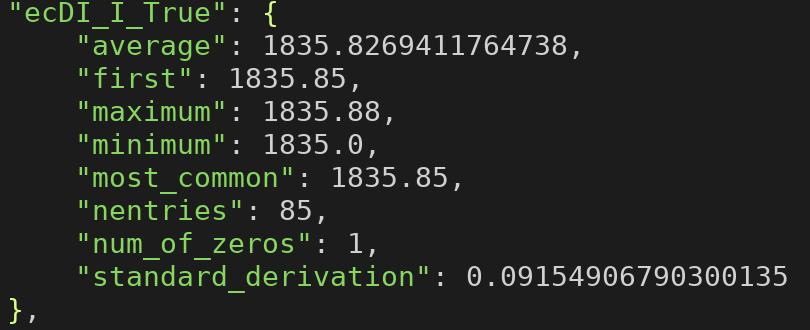
\includegraphics[width = \textwidth]{values_example.png}
%\end{block}
%\end{column}
%\begin{column}[T]{0.5\textwidth}
%\smaller
%EPICS values are read out once per 30 seconds. 
%\begin{itemize}
%    \item $nentries$ : # of read out
%    \item $num\_of\_zeros$ : sometimes it failed to read out, delete this zero in data set.  
%\end{itemize}
%\end{column}
%\end{columns}
%
%\begin{columns}
%\begin{column}[T]{0.5\textwidth}
%\begin{block}{for one run group}
%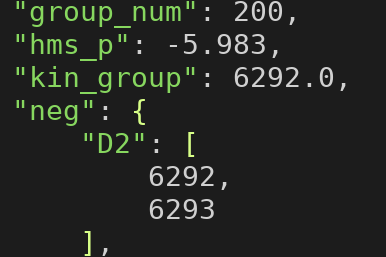
\includegraphics[width = 0.6\textwidth]{rungroup_zoomin.png}
%\end{block}
%\end{column}
%\begin{column}[T]{0.5\textwidth}
%\begin{itemize}
%    \item $average$ : average weighted by "nentries" 
%    \item $most_common$ : "most common" of the run with largest nentries. 
%    \item $stdder$ : standard derivation weighted by nentries
%\end{itemize}
%\end{column}
%\end{columns}
%\end{frame}
%
%\begin{frame}{ratio definition}
%\begin{columns}
%\begin{column}[T]{0.5\textwidth}
%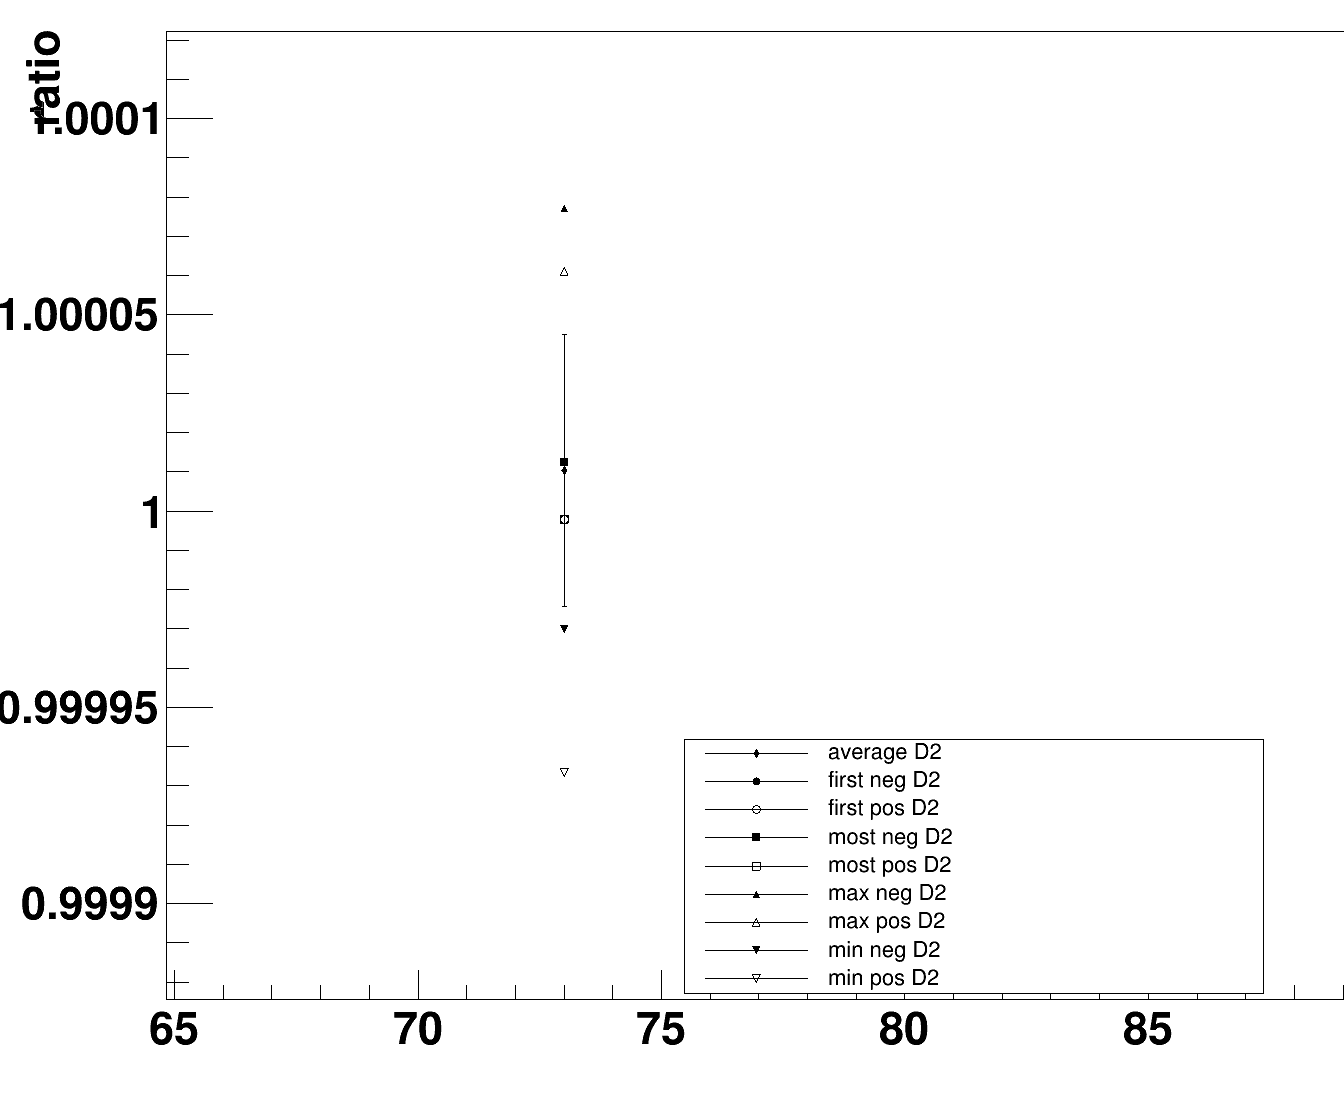
\includegraphics[width = \textwidth]{epicvaluezoomin.png}
%
%\end{column}
%\begin{column}[T]{0.5\textwidth}
%\begin{itemize}
%\smaller
%    \item ratio = $\frac{{value_{neg}}} {{value_{pos}}}$
%    \item average = $\frac{average_{neg}}{average_{pos}}$
%    \item first neg = $\frac{first_{neg}}{average_{pos}}$,first pos = $\frac{average_{neg}}{first_{pos}}$
%    \item most = similar to first
%    \item max neg = $\frac{max_{neg}}{average_{pos}}$
%    \item max pos = $\frac{average_{neg}}{min_{pos}}$
%    \item min neg = $\frac{min_{neg}}{average_{pos}}$
%    \item min pos = 
%    $\frac{average_{neg}}{max_{pos}}$
%    \item stdder = $\sqrt{(\frac{average_{neg}}{average_{pos}})^2((\frac{stdder_{neg}}{average_{neg}})^2+(\frac{stdder_{pos}}{average_{pos}})^2)}$
%\end{itemize}{}
%\end{column}
%\end{columns}
%\end{frame}


%\begin{frame}
%  \includegraphics[width = \textwidth]{graphs/hardware/SHMS_Layout_new.pdf}
%  %\includegraphics[width = \textwidth,trim=5mm 4cm 24.5cm 5mm,clip]{hardware/SHMS_Layout_new.pdf}
%\end{frame}
%
%
%\begin{frame}{ecQ2\_I\_True}
%    HMS magnet rs232 readback current
%    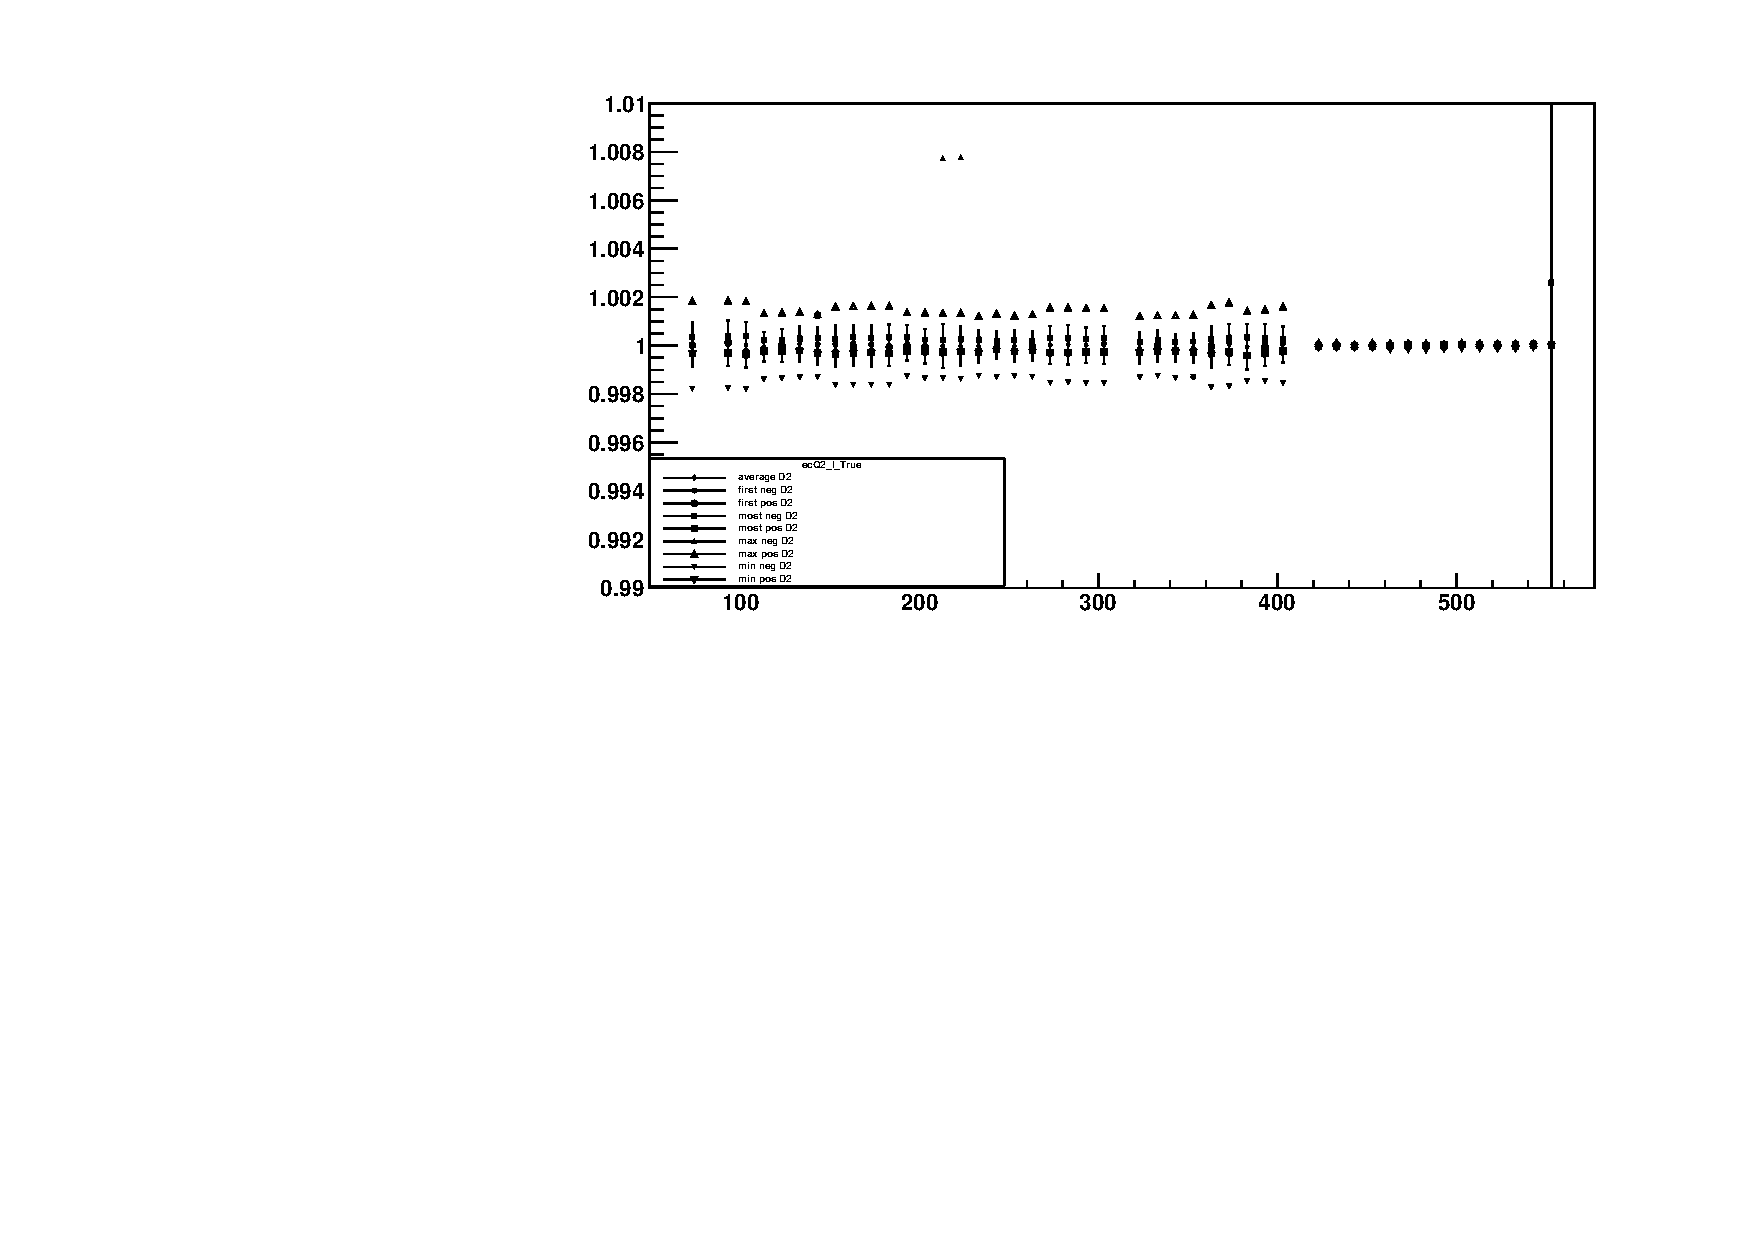
\includegraphics[width = \textwidth]{currentplot/ecQ2_I_True.pdf}
%\end{frame}
%
%\begin{frame}{ecQ2\_I\_coarse}
%   HMS magnet analog readback current
%   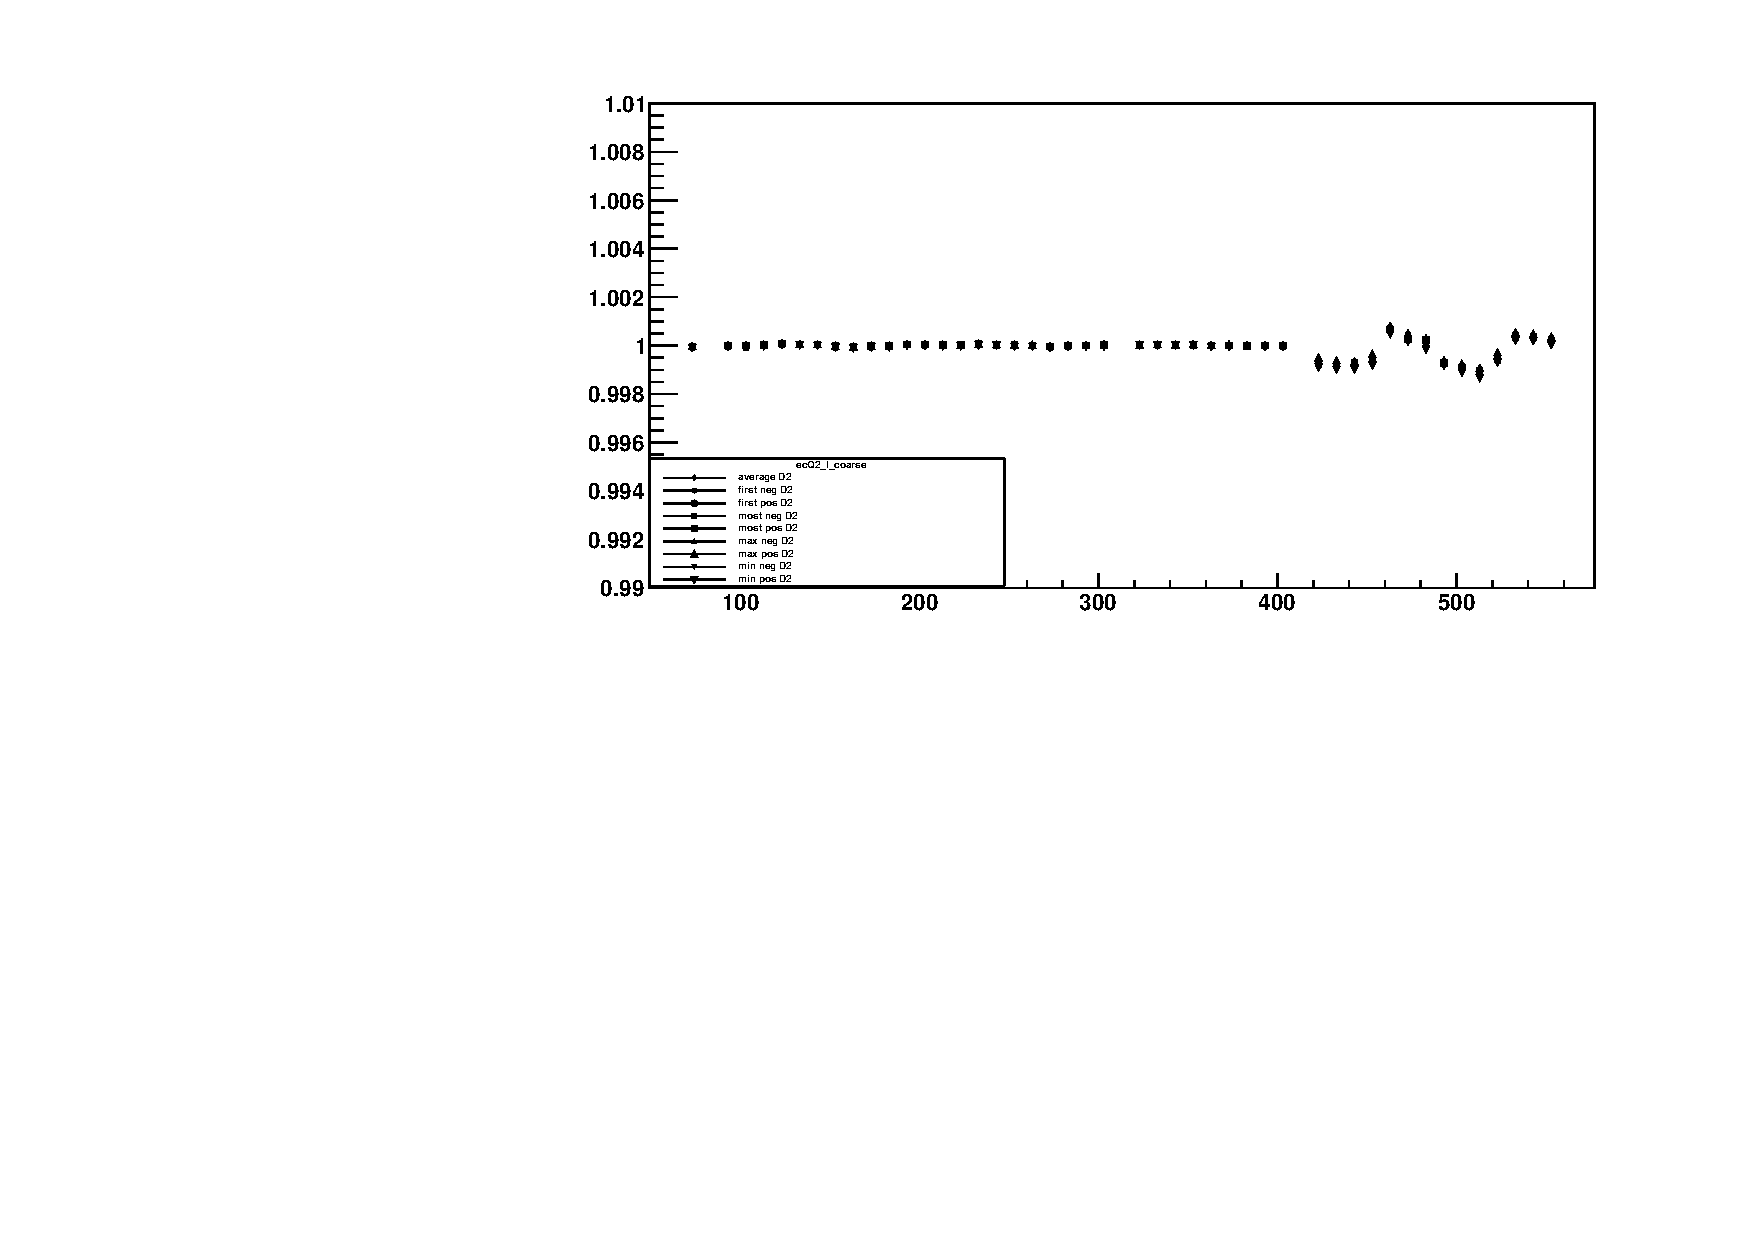
\includegraphics[width = \textwidth]{currentplot/ecQ2_I_coarse.pdf}
%   
%\end{frame}
%
%\begin{frame}{ecSQ2\_I\_True}
%    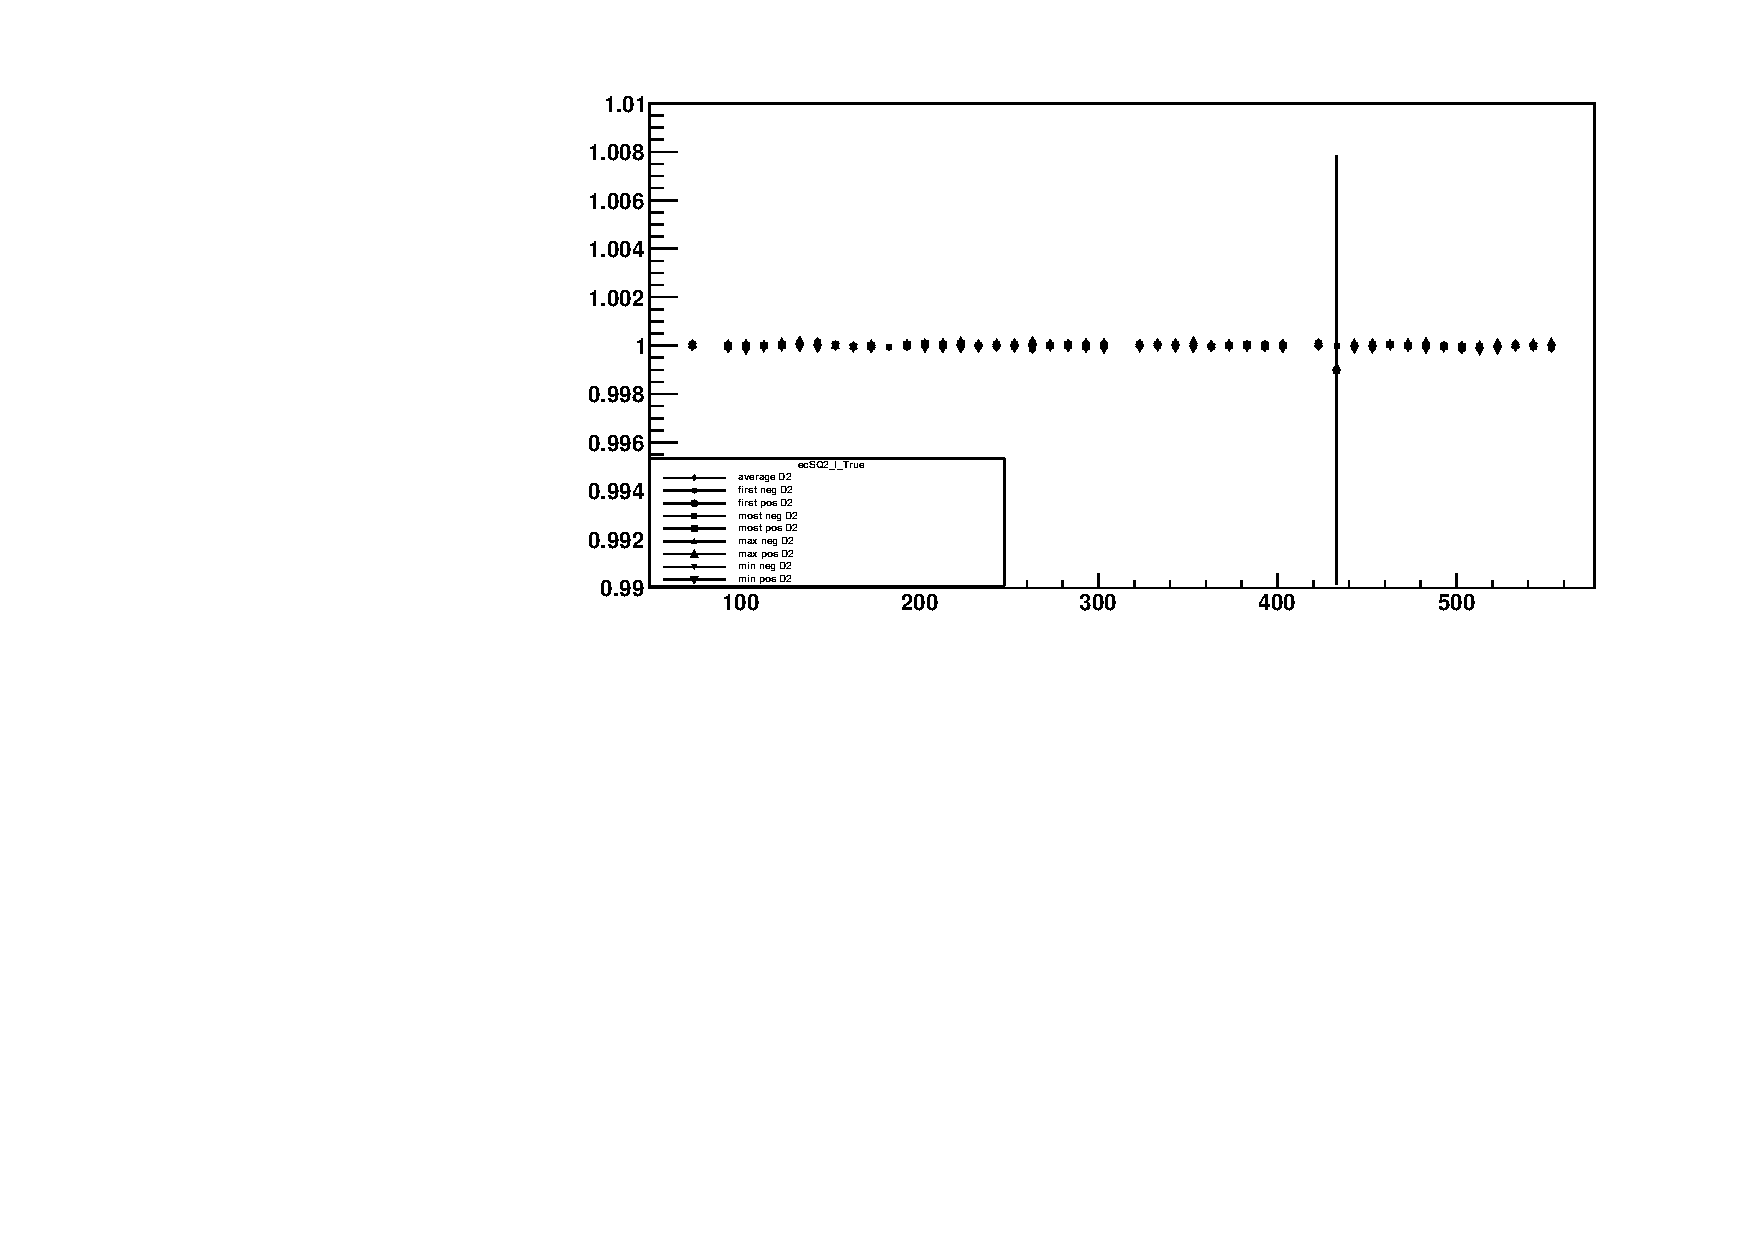
\includegraphics[width = \textwidth]{currentplot/ecSQ2_I_True.pdf}
%\end{frame}
%
%\begin{frame}{ecSQ2\_I\_coarse}
%  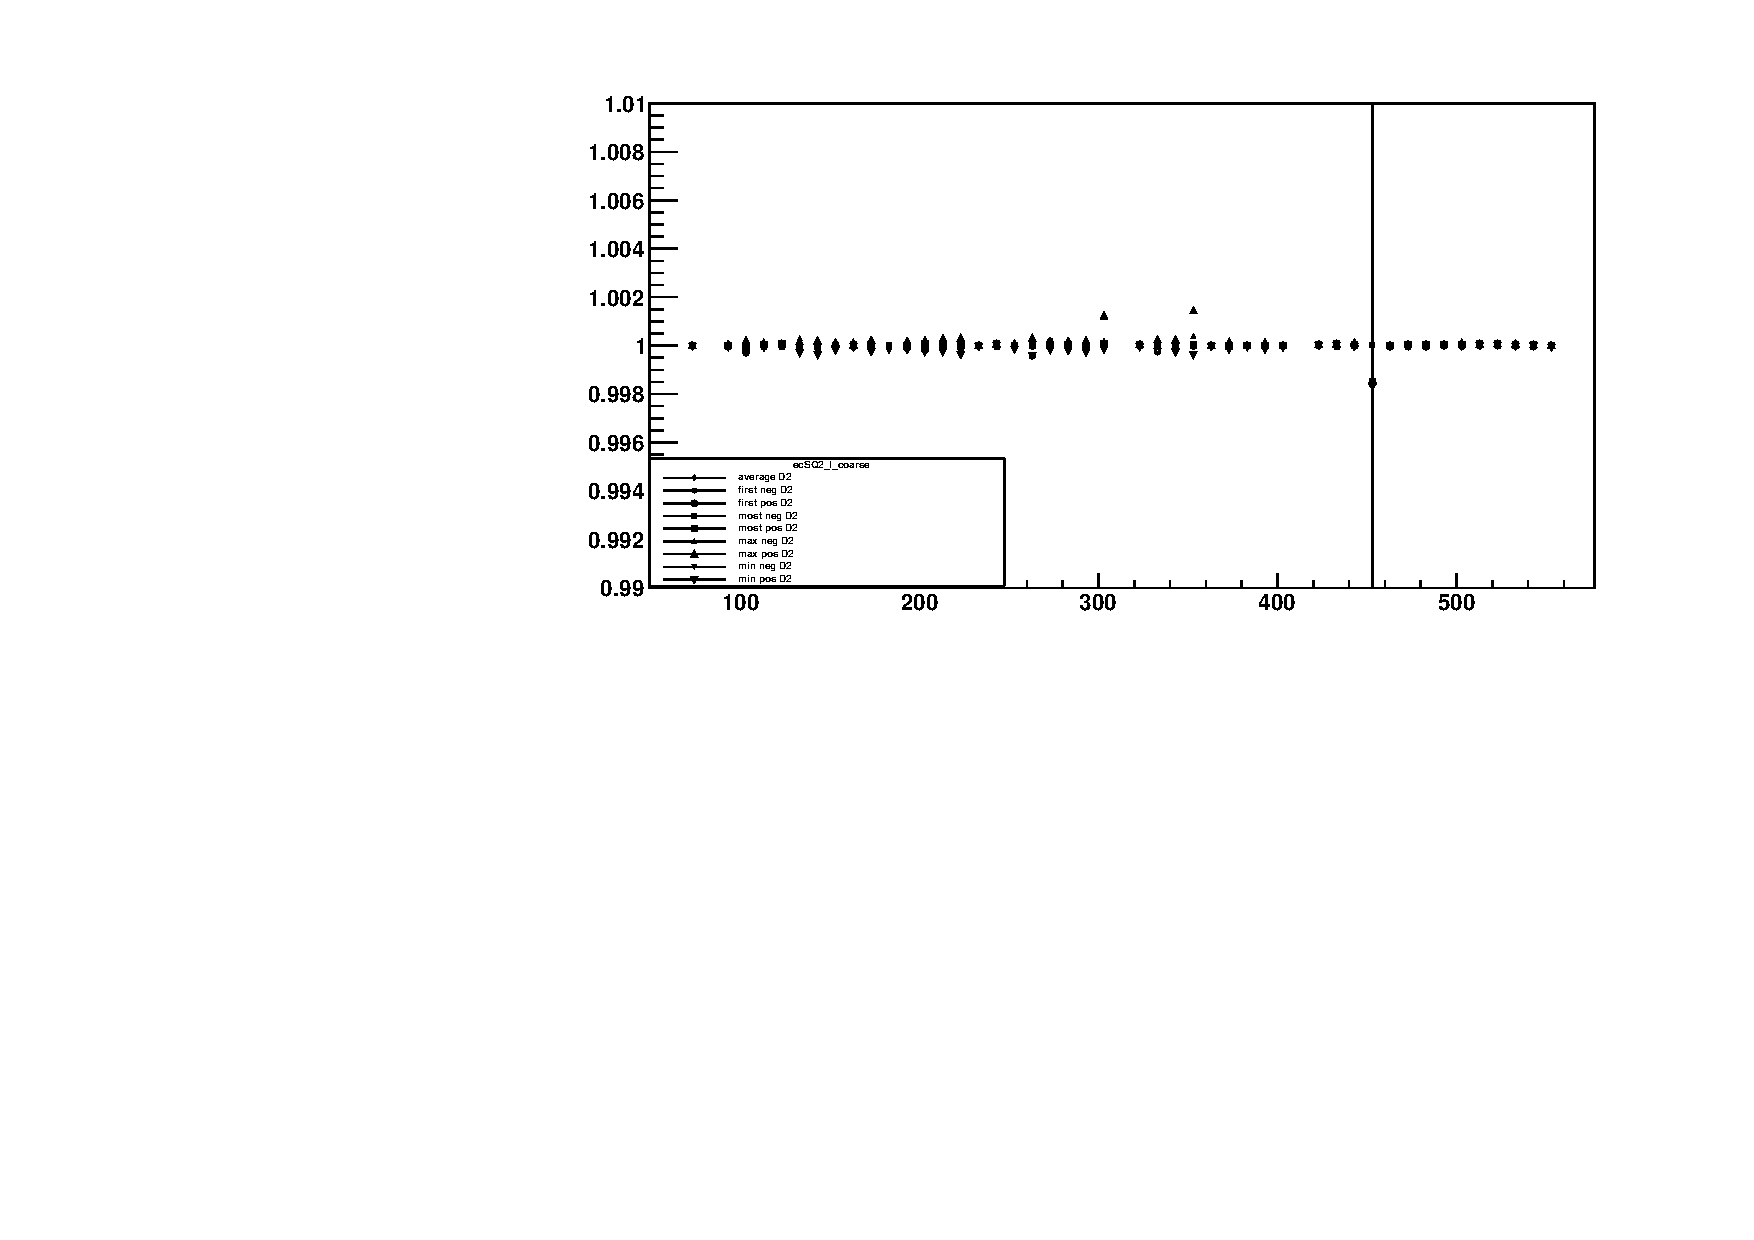
\includegraphics[width = \textwidth]{currentplot/ecSQ2_I_coarse.pdf}
%   
%\end{frame}
%
%%\begin{frame}{ecSDI\_B\_True\_NMR}
%%    SHMS dipole NMR readback
%%    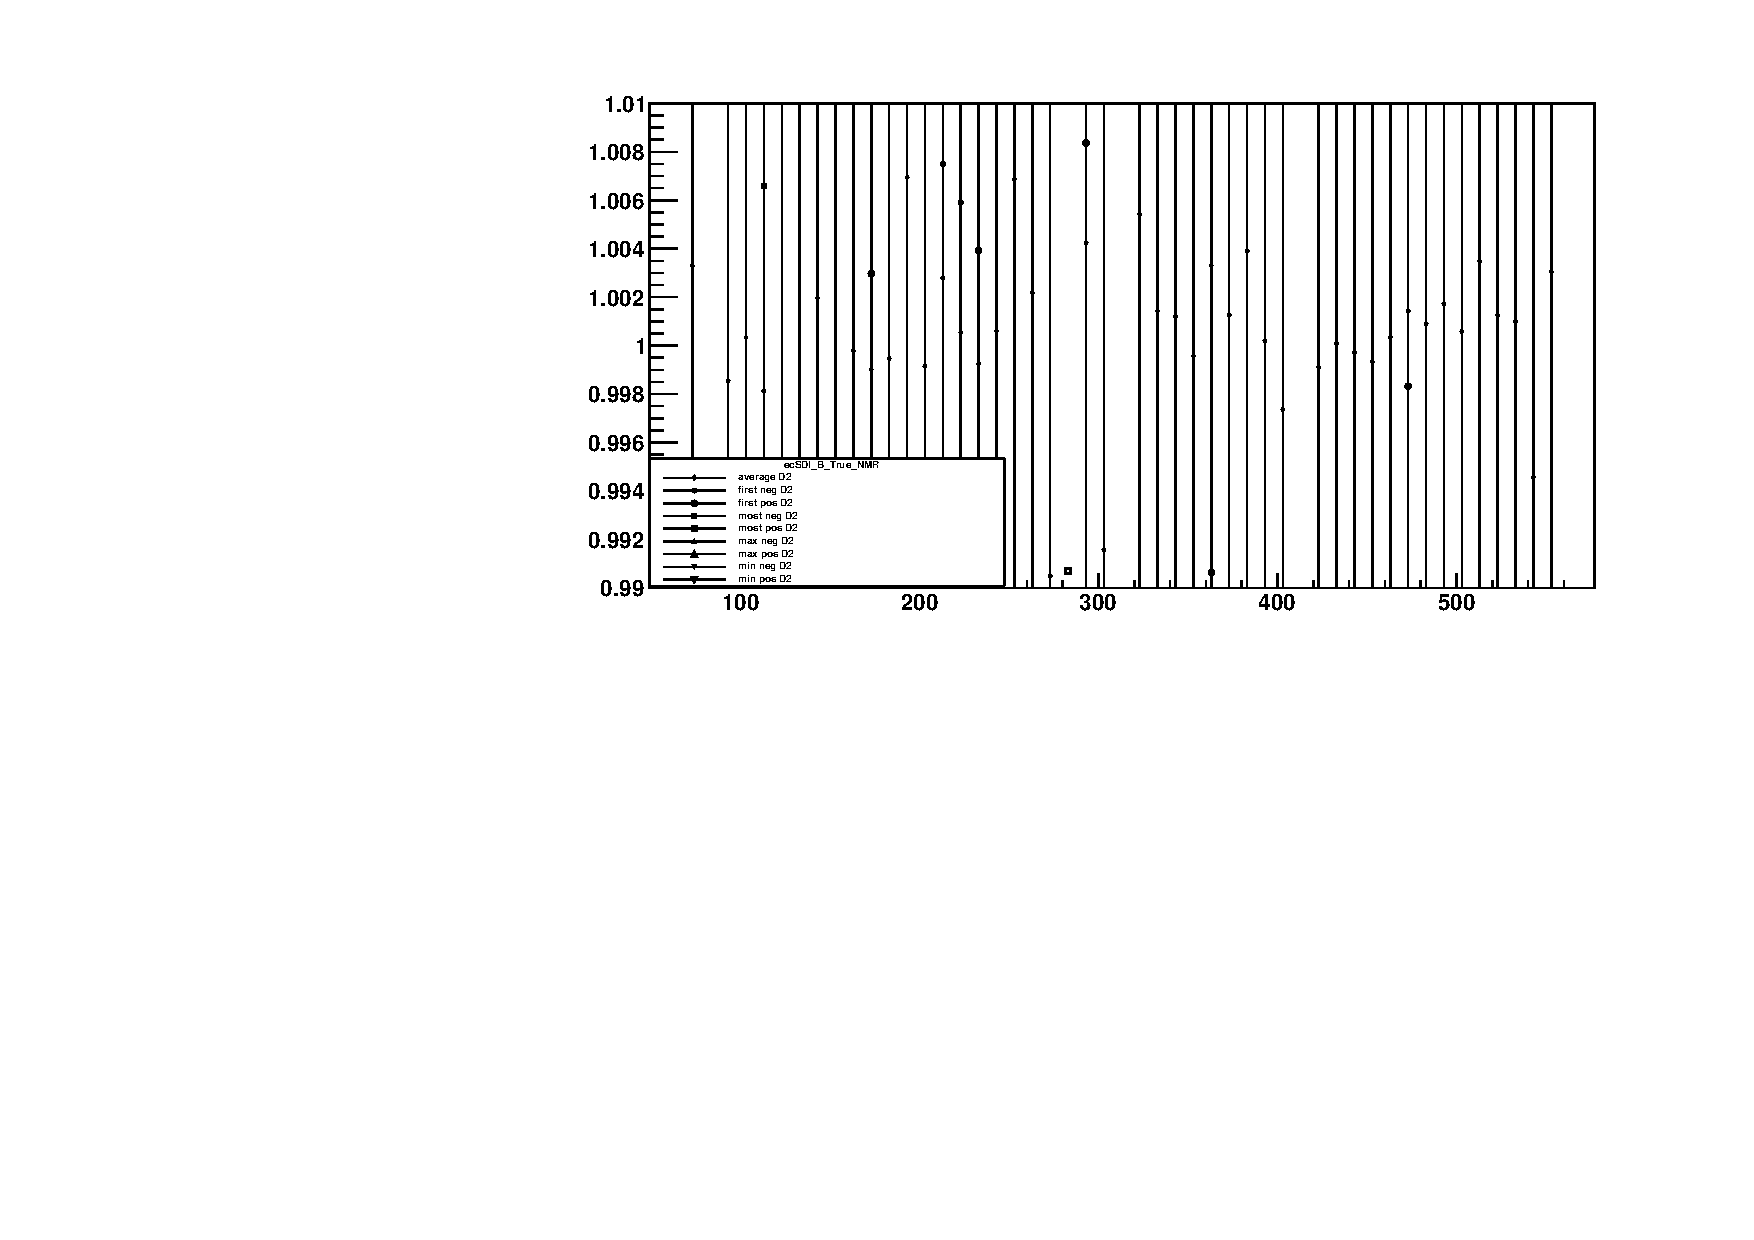
\includegraphics[width = \textwidth]{currentplot/ecSDI_B_True_NMR.pdf}
%%\end{frame}
%
%\begin{frame}{ecDI\+B\_Set\_NMR}
%  \begin{columns}
%    \begin{column}[T]{0.5\textwidth}
%  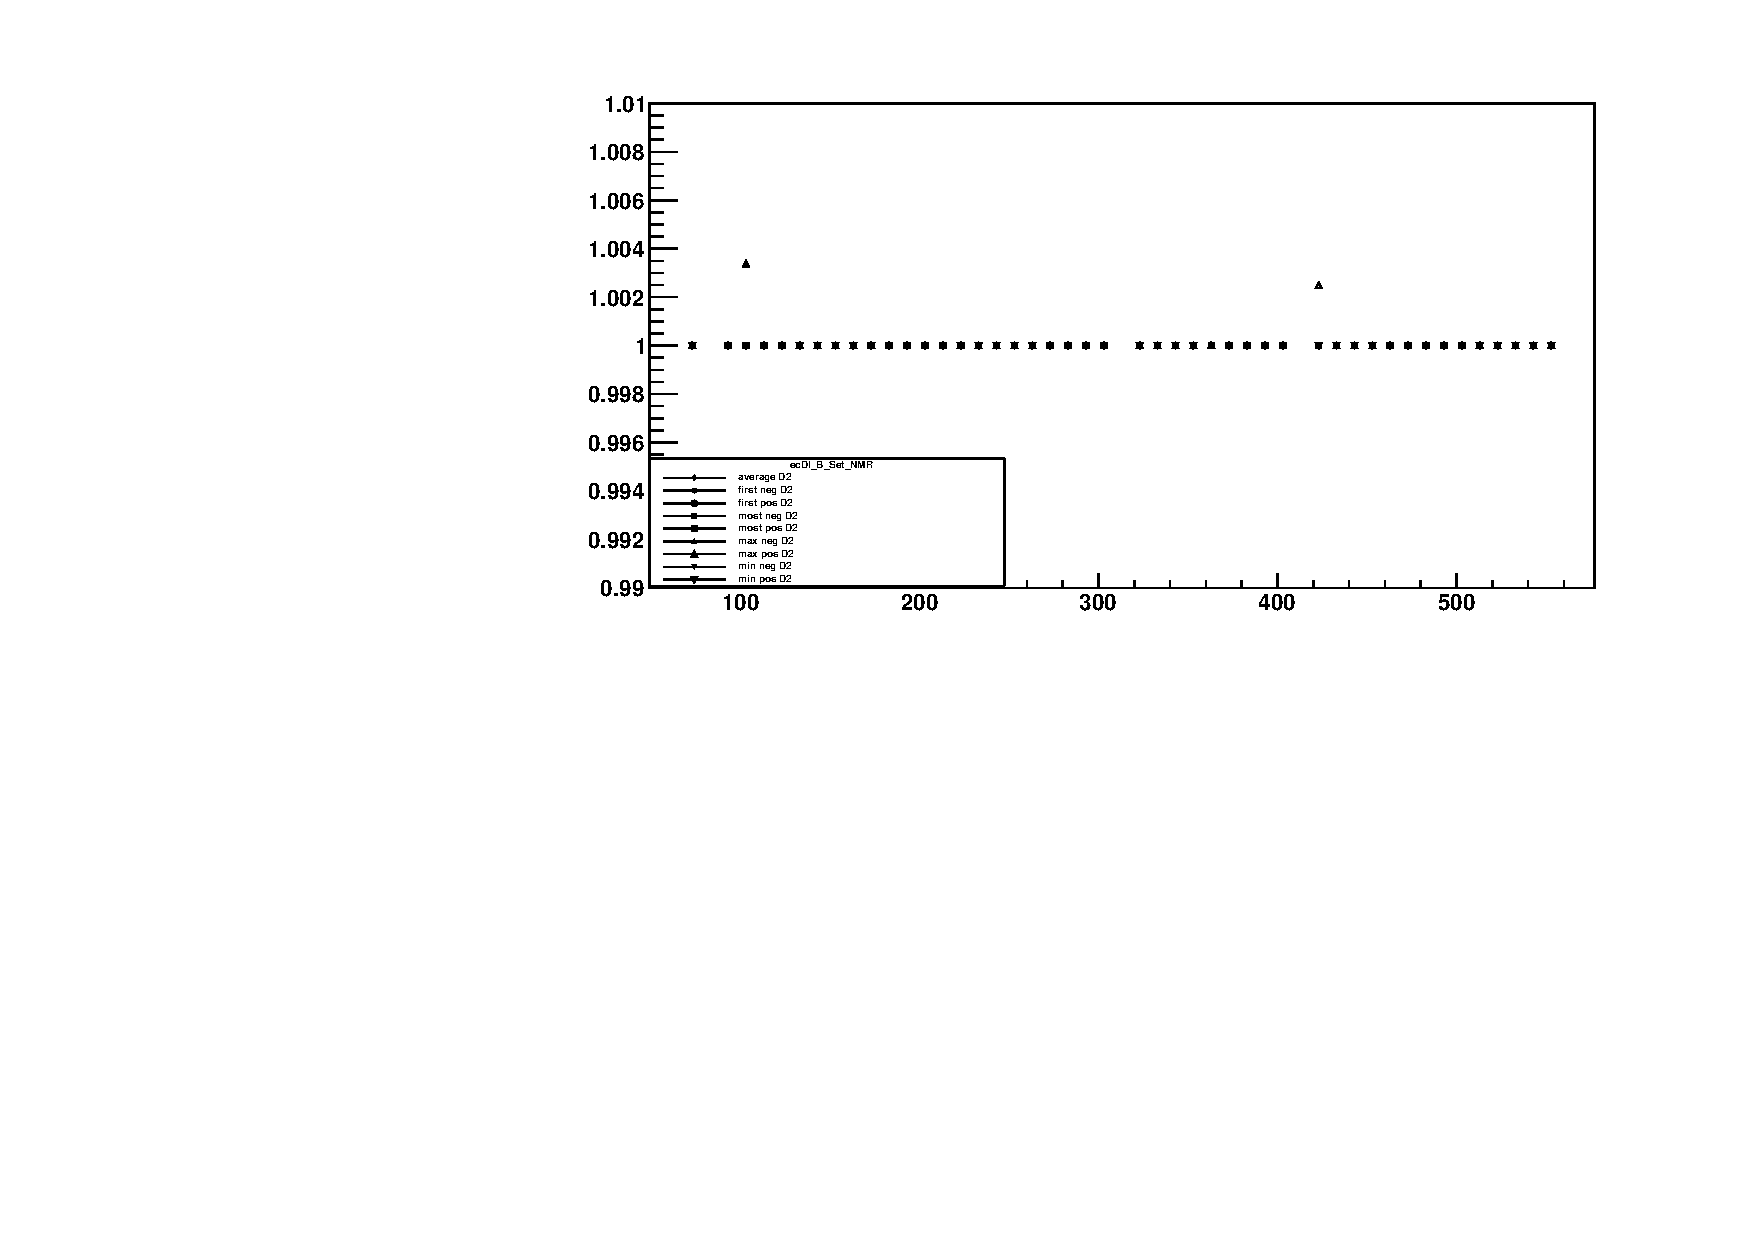
\includegraphics[width = \textwidth]{currentplot/ecDI_B_Set_NMR.pdf}
%\end{column}
%\begin{column}[T]{0.5\textwidth}
%HMS dipole NMR readback. Always 1.29
%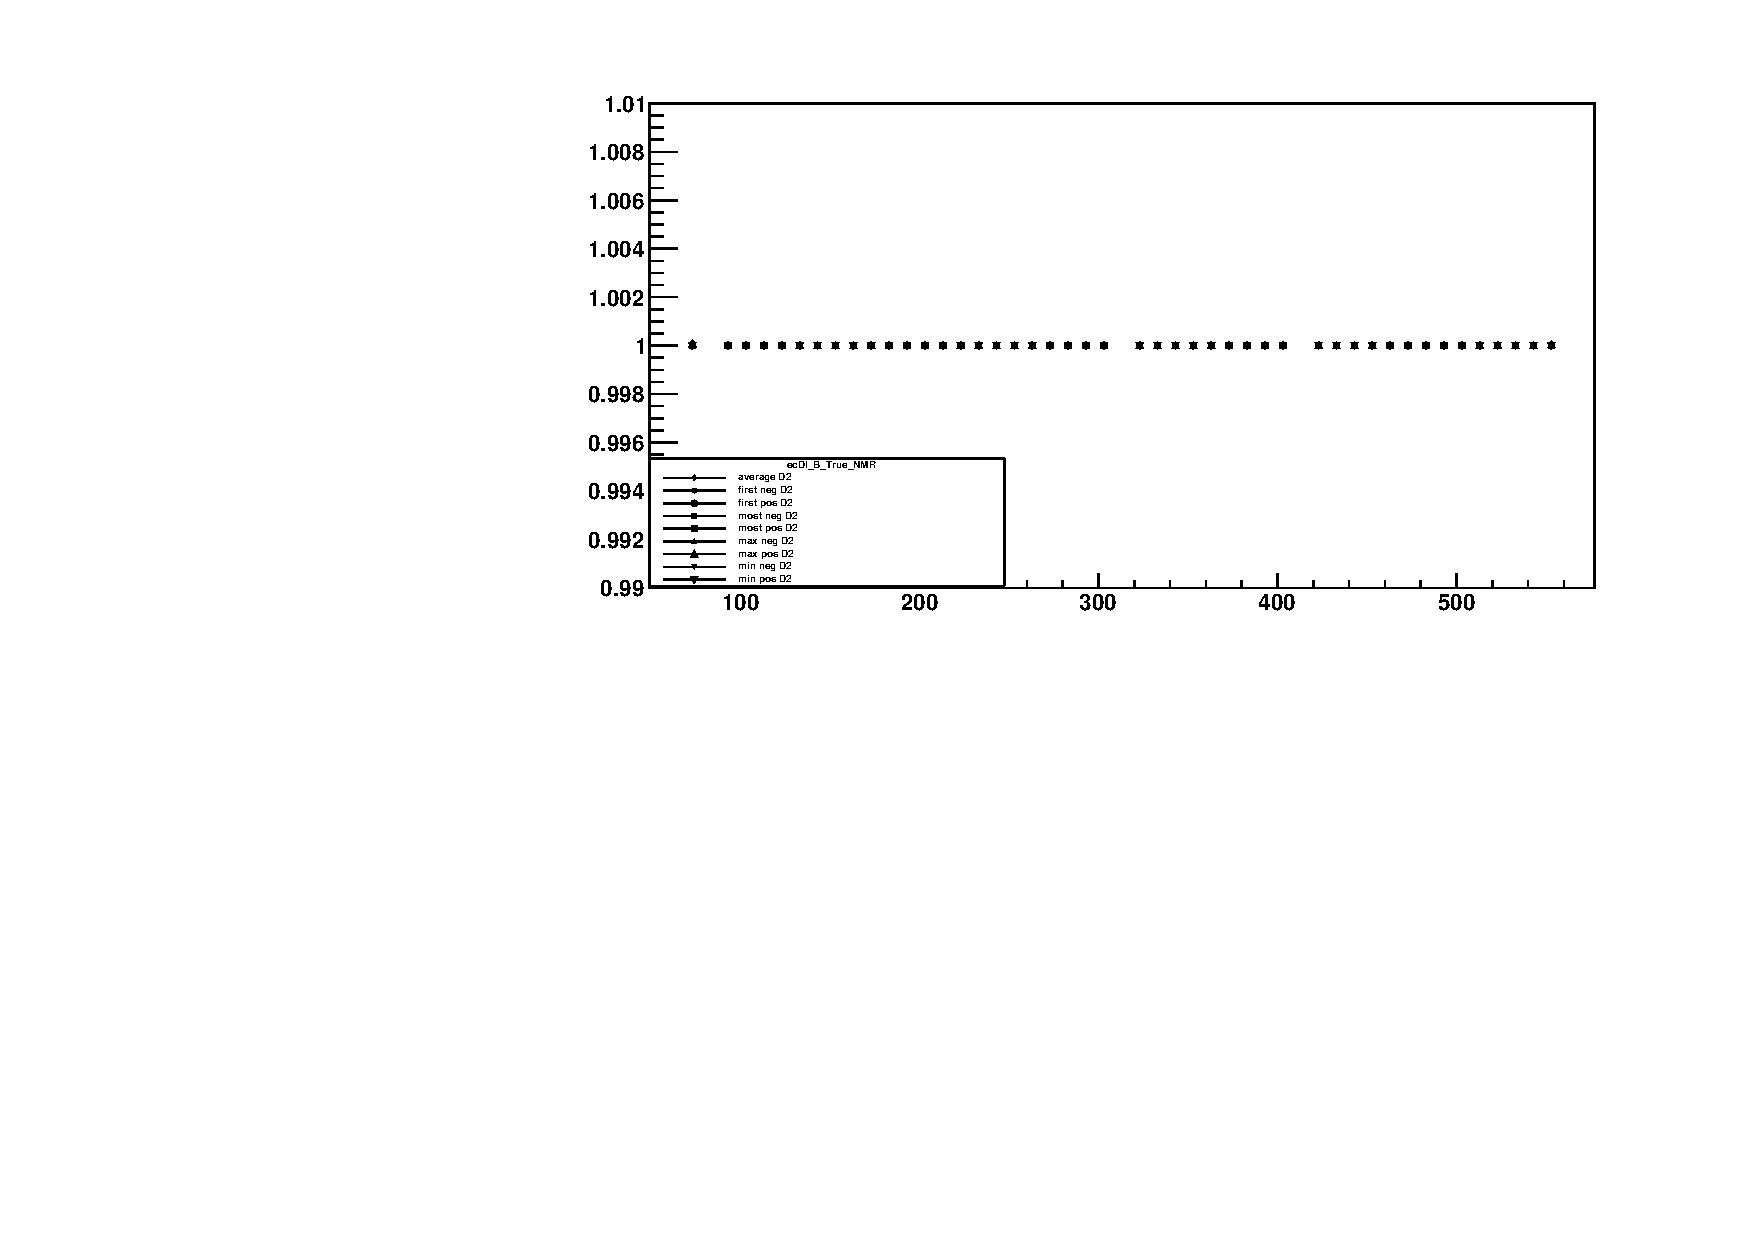
\includegraphics[width = \textwidth]{currentplot/ecDI_B_True_NMR.pdf}
%\end{column}
%\end{columns}
%\begin{columns}
%  \begin{column}[T]{0.5\textwidth}
%    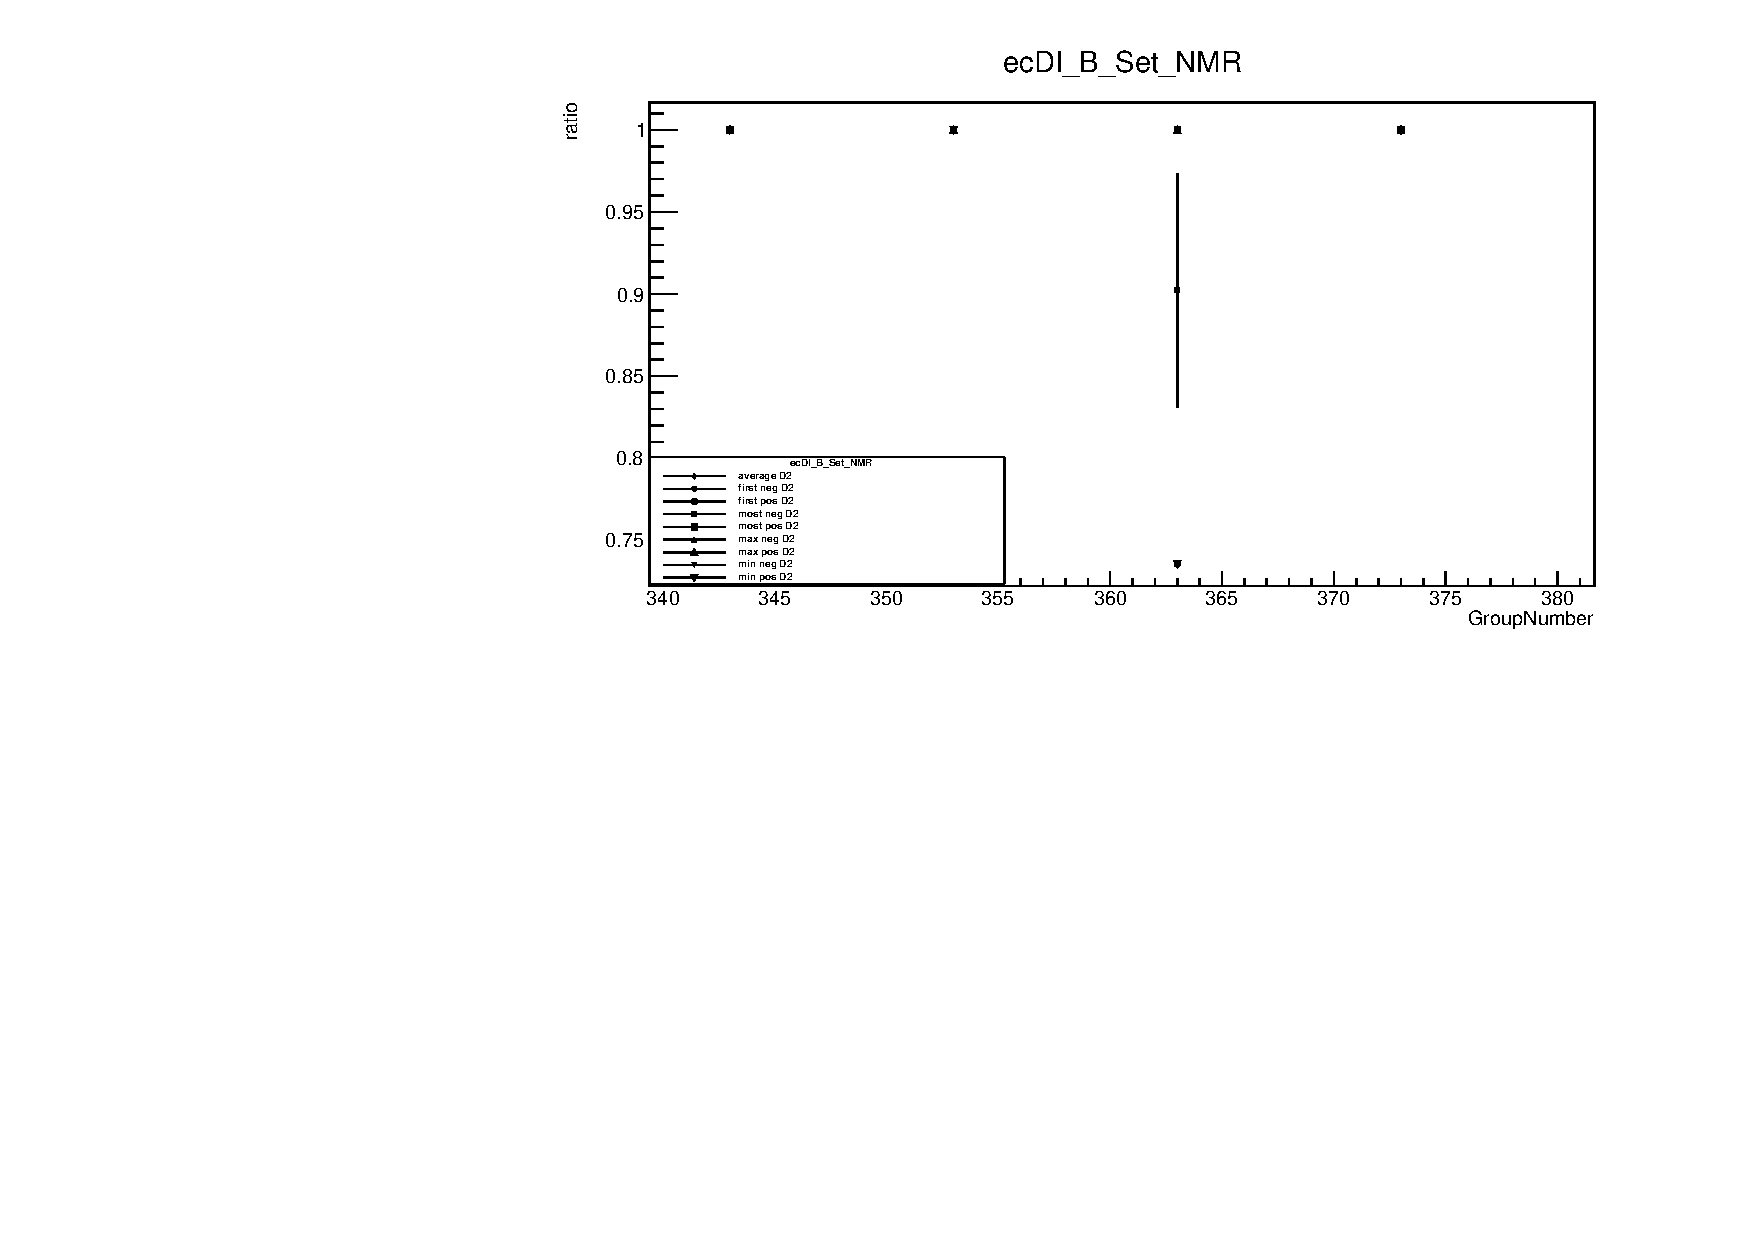
\includegraphics[width = \textwidth]{ecDI_B_Set_NMR_problem.pdf}
%
%    \end{column}
%  \begin{column}[T]{0.5\textwidth}
%     HMS dipole NMR set value, problem at group 360 for run 6519, half 1.76, later half 1.29, But 
%     HMS dipole true readback is stable, for 6519 it's 1.29
%  \end{column}
%  \end{columns}
%\end{frame}

\begin{frame}{HP,HallP}
    \begin{block}{pattern: up}
    ecSDI\_HP : SHMS HP raw Hall probe value
    
    ecSHB\_HP : SHMS HB raw Hall probe value
    
    ecSHB\_HallP : SHMS Hall probes HB(corrected) 
    
    ecSQ3\_HP : SHMS Q3 raw Hall probe value
    
    ecSQ3\_HallP: SHMS Hall probes Q3(corrected)
    \end{block}
    \begin{block}{pattern: down}
    ecsQ1\_HP : SHMS Q1 raw Hall probe value
    
    ecsQ1\_HallP : SHMS Hall probes Q1(corrected)
    
    ecsQ2\_HP : SHMS Q2 raw Hall probe value
    
    ecsQ2\_HallP :SHMS Hall probes Q2(corrected)
    \end{block}
There is a pattern going along with z.     
    
    
\end{frame}

\begin{frame}{ecSHB\_HallP}
    SHMS Hall probes HB (corrected)
    \includegraphics[width = \textwidth]{currentplot/ecSHB_HallP_all.pdf}
\end{frame}


\begin{frame}{ecSHB\_HallP}
    \begin{columns}
    \begin{column}[T]{0.5\textwidth}
    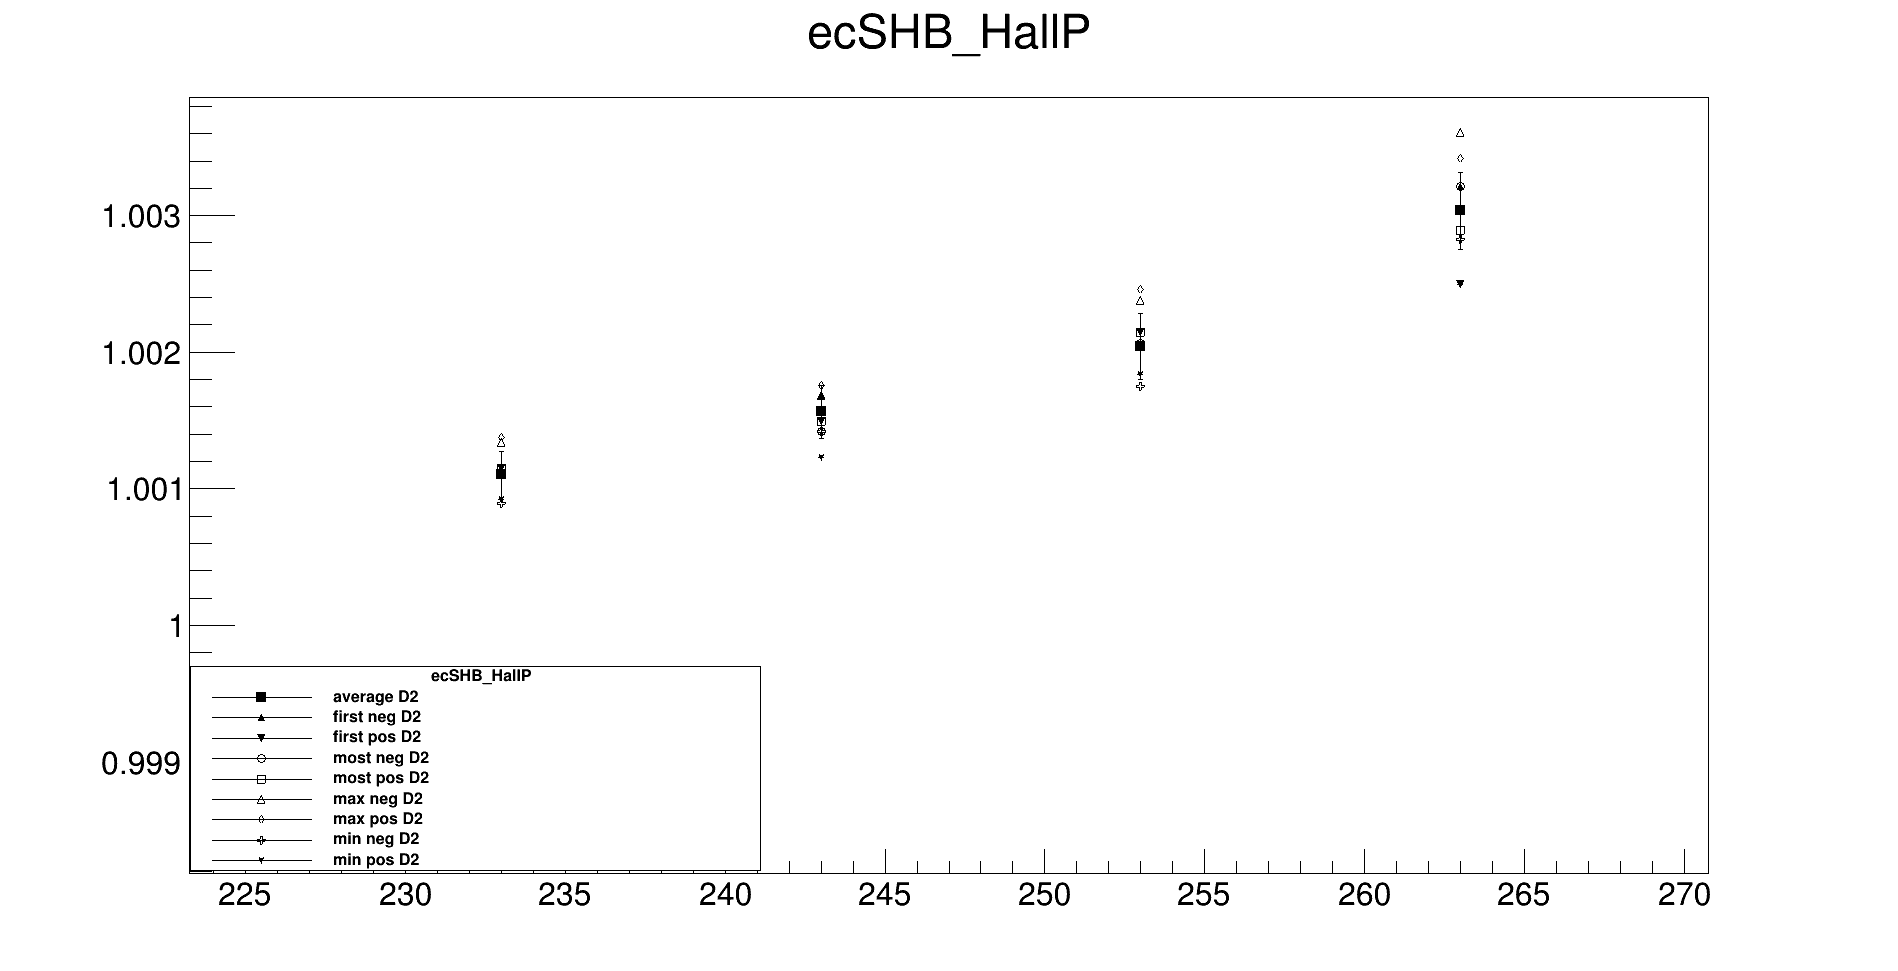
\includegraphics[width = \textwidth]{ecSHB_HallP_zoomin.png}
    \end{column}
    \begin{column}[T]{0.5\textwidth}
      \smaller  
    \begin{itemize}
      \item $hms\_P$ = -6.358
        \item $230$ : 6359-6365, shms\_P = -2.966,z = 0.7
        \item $240$ : 6367-6372, shms\_P = -2.541,z = 0.6
        \item $250$ : 6373-6377, shms\_P = -2.116,z = 0.5
        \item $260$ : 6378-6383, shms\_P = -1.691,z = 0.4
    \end{itemize}
    \end{column}
    \end{columns}
\begin{columns}
\begin{column}[T]{0.5\textwidth}
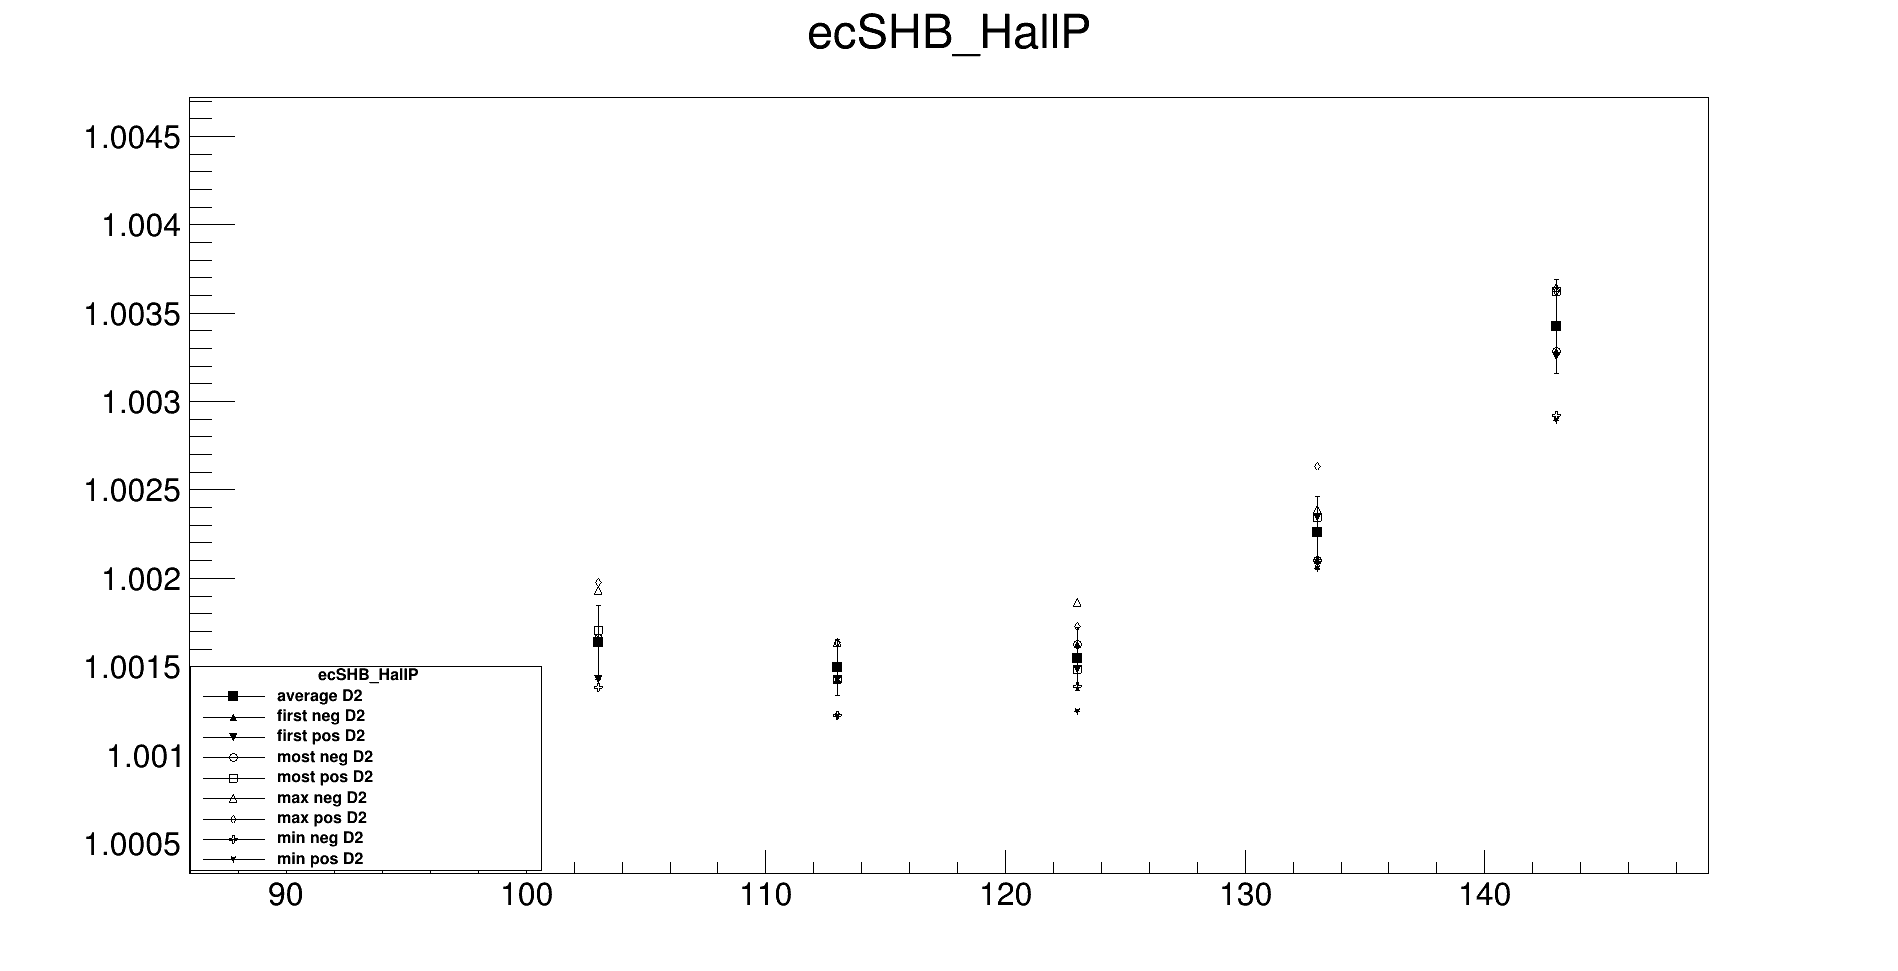
\includegraphics[width = \textwidth]{ecSHB_HallP_zoomin2.png}
\end{column}
\begin{column}[T]{0.5\textwidth}
\smaller
\begin{itemize}
    %\item $100$ : 6049-6064, hms\_P = -4.508, shms\_P = 2.433
  \item $hms\_P$ : -5.983
    \item $110$ : 6104-6114, shms\_P = -3.229, z = 0.7
    \item $120$ : 6115-6121, shms\_P = -2.767, z = 0.6
    \item $130$ : 6122-6128, shms\_P = -2.304, z = 0.5
    \item $140$ : 6129-6141, shms\_P = -1.842, z = 0.4
\end{itemize}
\end{column}
\end{columns}    
\end{frame}

%\begin{frame}{ecSDI\_HP}
%  ecSDI\_HP is for SHMS Dipole Magnet field raw value. SHMS Dipole Magnet field (corrected) doesn't exist, Why not? 
%\end{frame}



\begin{frame}{ecSQ1\_HallP}
SHMS Q1 Hall probe value corrected
    \includegraphics[width = \textwidth]{currentplot/ecSQ1_HallP.pdf}
\end{frame}

%\begin{frame}{ecSQ1\_HallP}
%\begin{columns}
%\begin{column}[T]{0.5\textwidth}
%  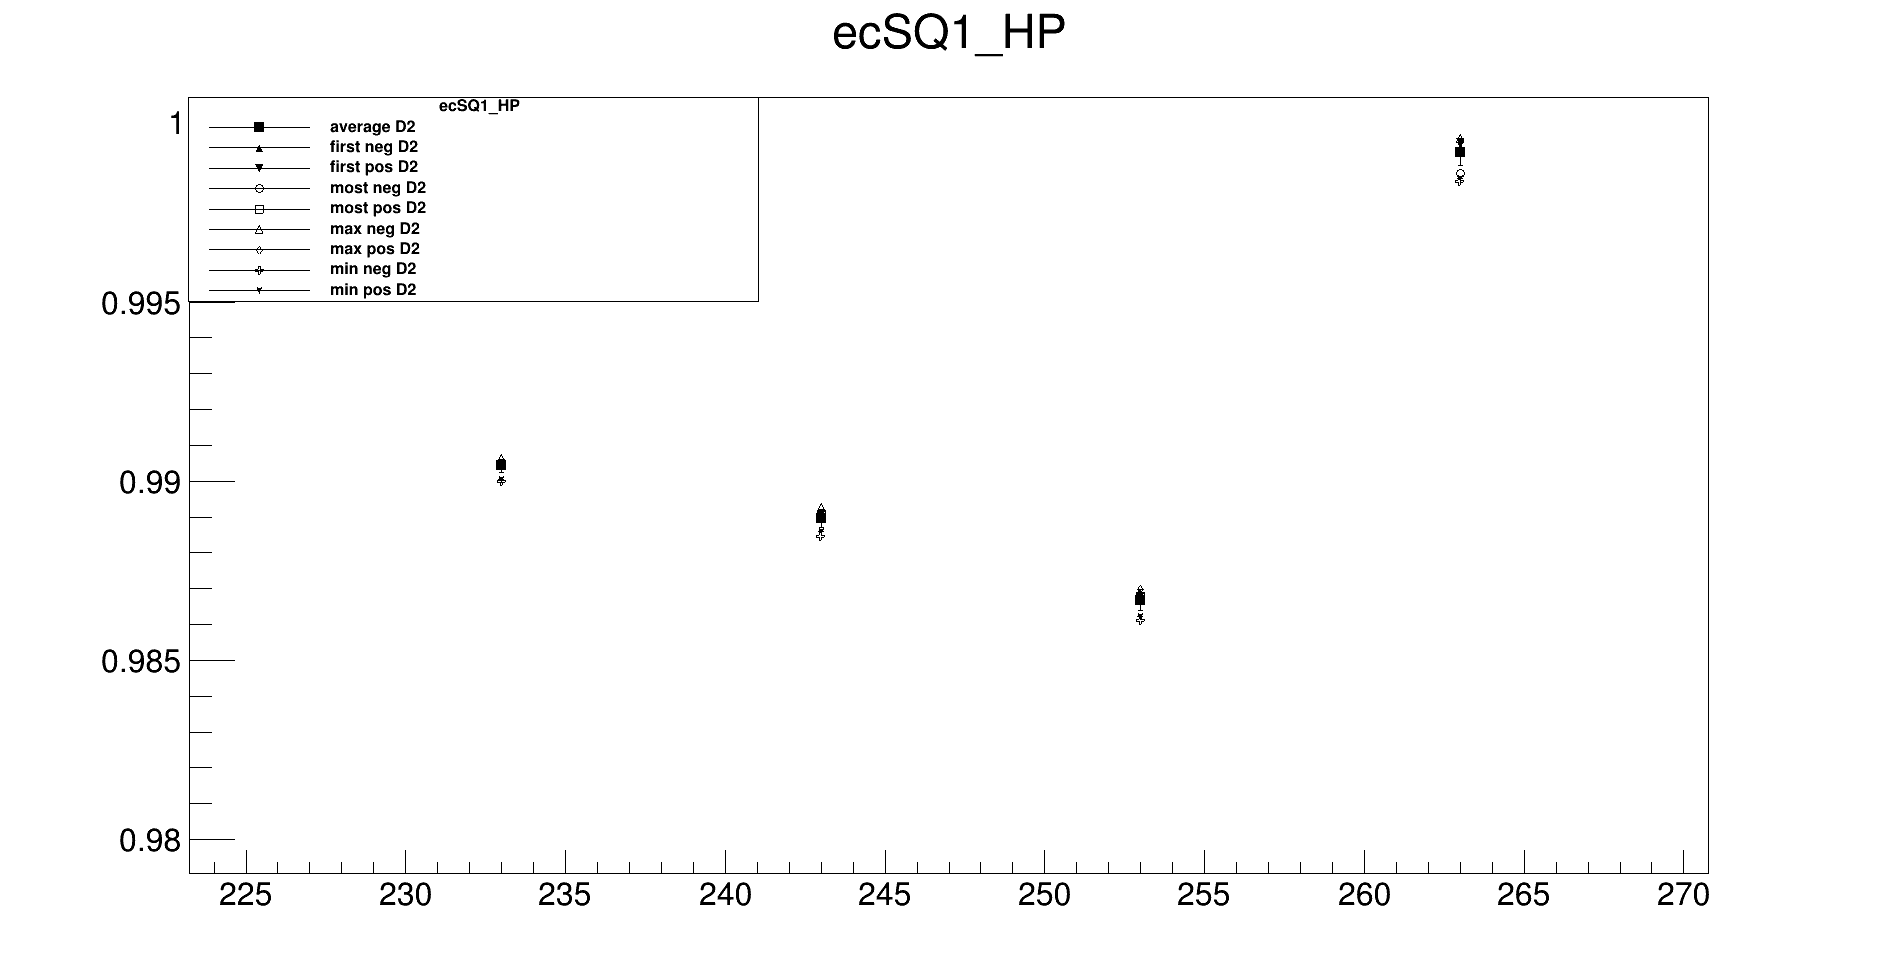
\includegraphics[width = \textwidth]{ecSQ1_HP_zoomin1.png}
%\end{column}
%\begin{column}[T]{0.5\textwidth}
%      \smaller  
%\begin{itemize}
%        \item $hms\_P$ = -6.358
%        \item $230$ : 6359-6365, shms\_P = -2.966,z = 0.7
%        \item $240$ : 6367-6372, shms\_P = -2.541,z = 0.6
%        \item $250$ : 6373-6377, shms\_P = -2.116,z = 0.5
%        \item $260$ : 6378-6383, shms\_P = -1.691,z = 0.4
%    \end{itemize}
%\end{column}
%\end{columns}
%\begin{columns}
%\begin{column}[T]{0.5\textwidth}
%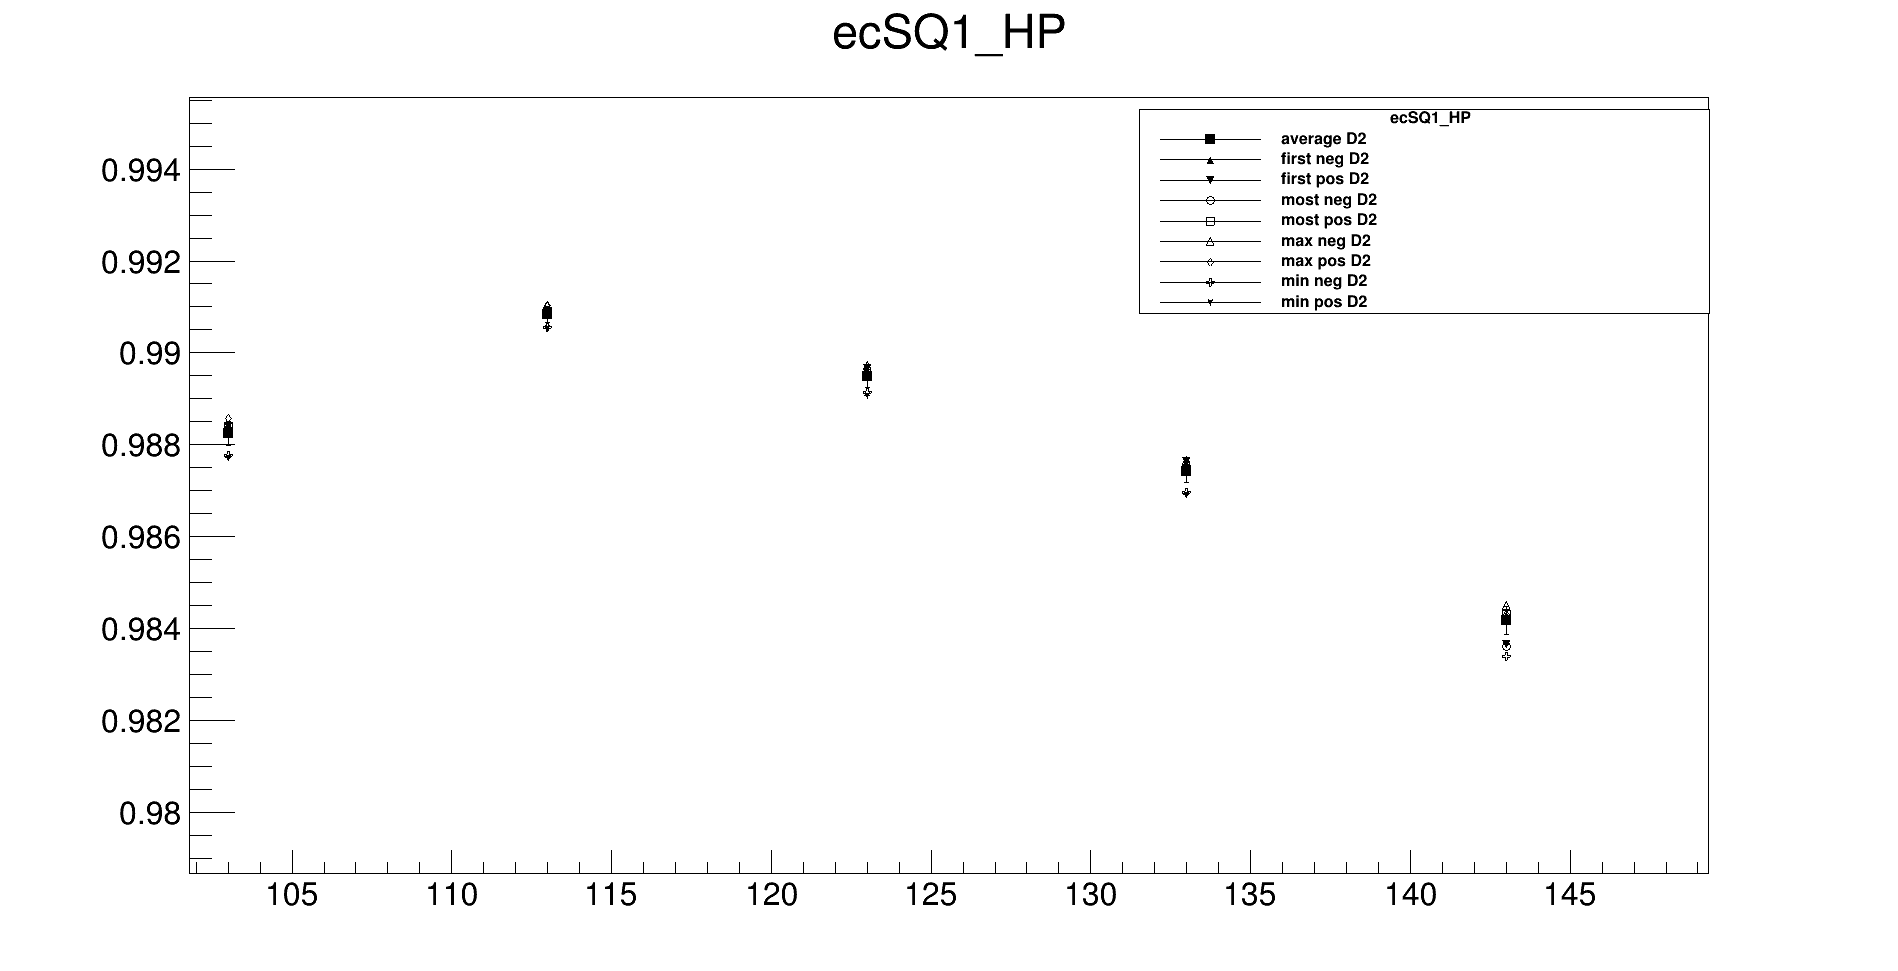
\includegraphics[width = \textwidth]{ecSQ1_HP_zoomin.png}
%\end{column}
%\begin{column}[T]{0.5\textwidth}
%%\item $100$ : 6049-6064, hms\_P = -4.508, shms\_P = 2.433
%    \item $hms\_P$: -5.983
%    \item $110$ : 6104-6114, shms\_P = -3.229, z = 0.7
%    \item $120$ : 6115-6121, shms\_P = -2.767, z = 0.6
%    \item $130$ : 6122-6128, shms\_P = -2.304, z = 0.5
%    \item $140$ : 6129-6141, shms\_P = -1.842, z = 0.4
%\end{column}
%\end{columns}   
%\end{frame}

\begin{frame}{kinematics}
  \begin{figure}
  \begin{overpic}[width = 0.9\textwidth]{graphs/kinematics_neg.png}
    \put(75,41){\includegraphics[width = 0.23\textwidth]{graphs/kinlegend.png}}
\end{overpic}  
\end{figure}
\end{frame}

\begin{frame}{group 140 kinematics}
  Choose all positive and negative polarity runs in run group 140, Q2 = 3.898, x = 0.45, shms_p 1.842, hms_p -5.983
  \begin{columns}
    \begin{column}[T]{0.5\textwidth}
      negative for pi-
      \includegraphics[width = \textwidth]{kin_acceptance/x_Q2_neg_140.pdf}
  \end{column}
  \begin{column}[T]{0.5\textwidth}
    positive for pi+
    \includegraphics[width = \textwidth]{kin_acceptance/x_Q2_pos_140.pdf}
  \end{column}
\end{columns}
\end{frame}

\begin{frame}{Change coordinate system}
  \begin{columns}
    \begin{column}[T]{0.5\textwidth}
  \includegraphics[width = \textwidth]{graphs/mydrawing/xyz_target_shms.pdf}
\end{column}
\begin{column}[T]{0.5\textwidth}
  Rotate along z for \pi /2
  
  Rotate along x for shms angle
    $\vec{p}_{beamline} = (P.gtr.px,P.gtr.py,P.gtr.pz)$
    \\
    $\mathcal{R} = \mathcal{R}_x *\mathcal{R}_z$
    \\
   $ \mathcal{R} = 
    \begin{bmatrix}
      0 & -1 & 0 \\
      cos(\theta) & 0 & -sin(\theta) \\
      sin(\theta) & 0 & cos(\theta)
    \end{bmatrix}
 $
    \\
    $\vec{p}_{spectrometer} = \mathcal{R}*\vec{p}_{beamline}$
\end{column}
\end{columns}
\end{frame}

\begin{frame}{group 140}
  negative runs for rungroup 140
  \includegraphics[width = 0.8\textwidth]{kin_acceptance/kin_neg_acceptance_140.png}
\end{frame}

\begin{frame}
  positive runs for run group 140
  \includegraphics[width = 0.8\textwidth]{kin_acceptance/kin_pos_acceptance_140.png}
\end{frame}

\begin{frame}{group 140}
  \begin{columns}
    \begin{column}[T]{0.5\textwidth}
      negative for pi-
      \includegraphics[width = \textwidth]{kin_acceptance/kin_neg_acceptance_cuts140.png}
    \end{column}
    \begin{column}[T]{0.5\textwidth}
  %    positive for pi+
  %    \includegraphics[width = \textwidth]{kin_acceptance/kin_pos_acceptance_cuts140.png}
       \includegraphics[width = \textwidth]{graphs/Empirical_Rule.PNG}
       \\
       cut1: 68\%, cut2: 95\%,cut3: 99.7\% 
    \end{column}
  \end{columns}

\end{frame}

\begin{frame}{xbj for group 140 pi- runs}
  for negative run 
  \begin{columns}
    \begin{column}[T]{0.5\textwidth}
      compare xbj without cut and after cut1
      \includegraphics[width = 0.8\textwidth]{kin_acceptance/xbj_neg_xq2cut_cut1_140.png}
\end{column}
\begin{column}[T]{0.5\textwidth}
  compare xbj after cut3 and cut1
  \includegraphics[width = 0.8\textwidth]{kin_acceptance/xbj_neg_cut3_cut1_140.png}
\end{column}
\end{columns}
\end{frame}

\begin{frame}{compare pi-&pi+ runs xbj for group 140}
      compare xbj for neg runs and pos runs
  \begin{columns}
    \begin{column}[T]{0.5\textwidth}
      no cut\\
      \includegraphics[width =0.7\textwidth]{kin_acceptance/compare_140_xbj_nocut.png}
\end{column}
\begin{column}[T]{0.5\textwidth}
cut1\\
  \includegraphics[width = 0.7\textwidth]{kin_acceptance/compare_140_xbj_cut1.png}
\end{column}
\end{columns}
  \begin{columns}
    \begin{column}[T]{0.5\textwidth}
       cut2\\
  \includegraphics[width =0.7\textwidth]{kin_acceptance/compare_140_xbj_cut2.png}
\end{column}
\begin{column}[T]{0.5\textwidth}
       cut3\\
  \includegraphics[width = 0.7\textwidth]{kin_acceptance/compare_140_xbj_cut3.png}
\end{column}
\end{columns}
\end{frame}

\begin{frame}{z for group 140 pi- runs}
  for negative runs
  \begin{columns}
    \begin{column}[T]{0.5\textwidth}
      compare z after xq2cut and cut1
      \includegraphics[width = 0.8\textwidth]{kin_acceptance/z_xq2cut_cut1_140.png}
\end{column}
\begin{column}[T]{0.5\textwidth}
  compare z after cut3 and cut1
  \includegraphics[width = 0.8\textwidth]{kin_acceptance/z_cut3_cut1_140.png}
\end{column}
\end{columns}
\end{frame}

\begin{frame}{compare pi-&pi+ runs z for group 140}
      compare z for neg runs and pos runs
  \begin{columns}
    \begin{column}[T]{0.5\textwidth}
      no cut\\
      \includegraphics[width =0.7\textwidth]{kin_acceptance/compare_140_z_nocut.png}
\end{column}
\begin{column}[T]{0.5\textwidth}
       cut1\\
  \includegraphics[width = 0.7\textwidth]{kin_acceptance/compare_140_z_cut1.png}
\end{column}
\end{columns}
  \begin{columns}
    \begin{column}[T]{0.5\textwidth}
       cut2\\
  \includegraphics[width =0.7\textwidth]{kin_acceptance/compare_140_z_cut2.png}
\end{column}
\begin{column}[T]{0.5\textwidth}
       cut3\\
  \includegraphics[width = 0.7\textwidth]{kin_acceptance/compare_140_z_cut3.png}
\end{column}
\end{columns}
\end{frame}

%spring
%  negative run for rungroup 440, hmsp -4.357, shms p -2.928
\begin{frame}
  negative run for rungroup 440, Q2 = 5.5, x = 0.65, hmsp -4.357, shms p -2.928
  \includegraphics[width = 0.8\textwidth]{kin_acceptance/kin_neg_acceptance_440.png}
\end{frame}

\begin{frame}
  positive runs for run group 440
  \includegraphics[width = 0.8\textwidth]{kin_acceptance/kin_pos_acceptance_440.png}
\end{frame}

\begin{frame}{group 440}
  \begin{columns}
    \begin{column}[T]{0.5\textwidth}
      negative for pi-
      \includegraphics[width = \textwidth]{kin_acceptance/kin_neg_acceptance_cuts440.png}
    \end{column}
    \begin{column}[T]{0.5\textwidth}
  %    positive for pi+
  %    \includegraphics[width = \textwidth]{kin_acceptance/kin_pos_acceptance_cuts440.png}
       \includegraphics[width = \textwidth]{graphs/Empirical_Rule.PNG}
       \\
       cut1: 68\%, cut2: 95\%,cut3: 99.7\% 
    \end{column}
  \end{columns}

\end{frame}

\begin{frame}{xbj for group 440 pi- runs}
  for negative run 
  \begin{columns}
    \begin{column}[T]{0.5\textwidth}
      compare xbj without cut and after cut1
      \includegraphics[width = 0.8\textwidth]{kin_acceptance/xbj_neg_xq2cut_cut1_440.png}
\end{column}
\begin{column}[T]{0.5\textwidth}
  compare xbj after cut3 and cut1
  \includegraphics[width = 0.8\textwidth]{kin_acceptance/xbj_neg_cut3_cut1_440.png}
\end{column}
\end{columns}
\end{frame}

\begin{frame}{compare pi-&pi+ runs xbj for group 440}
      compare xbj for neg runs and pos runs
  \begin{columns}
    \begin{column}[T]{0.5\textwidth}
      no cut\\
      \includegraphics[width =0.7\textwidth]{kin_acceptance/compare_440_xbj_nocut.png}
\end{column}
\begin{column}[T]{0.5\textwidth}
cut1\\
  \includegraphics[width = 0.7\textwidth]{kin_acceptance/compare_440_xbj_cut1.png}
\end{column}
\end{columns}
  \begin{columns}
    \begin{column}[T]{0.5\textwidth}
       cut2\\
  \includegraphics[width =0.7\textwidth]{kin_acceptance/compare_440_xbj_cut2.png}
\end{column}
\begin{column}[T]{0.5\textwidth}
       cut3\\
  \includegraphics[width = 0.7\textwidth]{kin_acceptance/compare_440_xbj_cut3.png}
\end{column}
\end{columns}
\end{frame}

\begin{frame}{z for group 440 pi- runs}
  for negative runs
  \begin{columns}
    \begin{column}[T]{0.5\textwidth}
      compare z after xq2cut and cut1
      \includegraphics[width = 0.8\textwidth]{kin_acceptance/z_xq2cut_cut1_440.png}
\end{column}
\begin{column}[T]{0.5\textwidth}
  compare z after cut3 and cut1
  \includegraphics[width = 0.8\textwidth]{kin_acceptance/z_cut3_cut1_440.png}
\end{column}
\end{columns}
\end{frame}

\begin{frame}{compare pi-&pi+ runs z for group 440}
      compare z for neg runs and pos runs
  \begin{columns}
    \begin{column}[T]{0.5\textwidth}
      no cut\\
      \includegraphics[width =0.7\textwidth]{kin_acceptance/compare_440_z_nocut.png}
\end{column}
\begin{column}[T]{0.5\textwidth}
       cut1\\
  \includegraphics[width = 0.7\textwidth]{kin_acceptance/compare_440_z_cut1.png}
\end{column}
\end{columns}
  \begin{columns}
    \begin{column}[T]{0.5\textwidth}
       cut2\\
  \includegraphics[width =0.7\textwidth]{kin_acceptance/compare_440_z_cut2.png}
\end{column}
\begin{column}[T]{0.5\textwidth}
       cut3\\
  \includegraphics[width = 0.7\textwidth]{kin_acceptance/compare_440_z_cut3.png}
\end{column}
\end{columns}
\end{frame}

\begin{frame}{Target}
\begin{columns}
\begin{column}[T]{0.5\textwidth}
\includegraphics[width = \textwidth]{graphs/hardware/target1.jpg}
\end{column}
\begin{column}[T]{0.5\textwidth}
\begin{itemize}
    \item $pressure 1$ : hcD2\_P\_Exhaust\_R, pressure loop D2 return
    \item $pressure 2$ : pressure loop D2 before, around 26 psia
    \item $temperature 1,2,3$ : Temperature at different position
    \item $density$ : read from NIST Chemistry WebBook
\end{itemize}
\end{column}
\end{columns}
\end{frame}

\begin{frame}{D2 status}
  \begin{columns}
    \begin{column}[T]{0.5\textwidth}
      \includegraphics[width = \textwidth]{currentplot/D2_P.pdf}
    \end{column}
    \begin{column}[T]{0.5\textwidth}
      \includegraphics[width = \textwidth]{currentplot/D2_T.pdf}
    \end{column}
\end{columns}
\end{frame}

\begin{frame}
  An example for LD2 density, this plot is density for D2 at temperature 22.33K, for different pressure(psia). 
  \includegraphics[width = \textwidth]{Target_fluid_property/D2_22d33K.png}

  \includegraphics[width = \textwidth]{graphs/NIST.png}
\end{frame}

\begin{frame}{D2}
  black dot for pi- runs, red dots for pi+ runs. 
   \includegraphics[width = 0.8\textwidth]{currentplot/D2_density.pdf}
\end{frame}

\begin{frame}{H2 status}
  \begin{columns}
    \begin{column}[T]{0.5\textwidth}
      \includegraphics[width = \textwidth]{currentplot/H2_P.pdf}
    \end{column}
    \begin{column}[T]{0.5\textwidth}
      \includegraphics[width = \textwidth]{currentplot/H2_T.pdf}
    \end{column}
\end{columns}
\end{frame}

\begin{frame}{H2}
     \includegraphics[width = 0.8\textwidth]{currentplot/H2_density.pdf}
\end{frame}

\begin{frame}{back up}
    Back Up
\end{frame}
\begin{frame}{group_num}
    \includegraphics[width = \textwidth]{group_num.png}
\end{frame}

\begin{frame}{kinematics_pos}
  \includegraphics[width = 0.8\textwidth]{graphs/kinematics_pos.png}
\end{frame}

\begin{frame}{6111xq2}
  \includegraphics[width = 0.8\textwidth]{kin_acceptance/6111xq2.png}
\end{frame}

\begin{frame}{pion momentum xy}
  \includegraphics[width = 0.8\textwidth]{kin_acceptance/pion_momentum_xy.png}
\end{frame}

\end{document}
 
